\documentclass[10pt,onecolumn,twoside,letterpaper]{article}
\usepackage[text={7in,9.5in},centering]{geometry}
\usepackage[spanish,es-nodecimaldot]{babel}

\usepackage{hyperref}

\usepackage{multicol}

\usepackage{harvard}% bibliographystyle: apsr, agsm, dcu, kluwer, nederlands

\usepackage{graphicx}
\usepackage{amssymb}
\usepackage{fancyhdr}
\usepackage{color}
\usepackage{colortbl}
\definecolor{gray}{cmyk}{0.0,0.0,0.0,0.60}

%\usepackage{auto-pst-pdf}
%\usepackage{pst-all}

%\usepackage[numbered]{mcode}
%\usepackage{lipsum}

\pagestyle{fancy}
\fancyhf{}
\fancyhead[RO]{\small{\textcolor{gray}{\textsc{Hacia un framework de locomoci\'on b\'ipeda evolutiva y flexible}}}}
\fancyhead[LO]{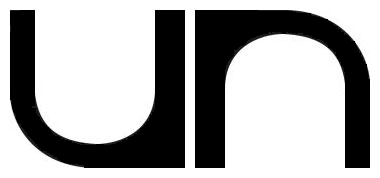
\includegraphics[scale=0.05]{../../images/unlogo.png}}
\fancyhead[LE]{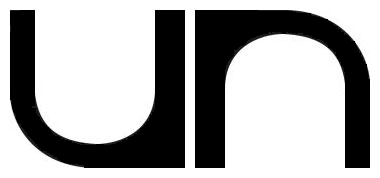
\includegraphics[scale=0.05]{../../images/unlogo.png}\quad\small{\textcolor{gray}{\textsc{Doctorado en ingenier\'ia: Mec\'anica y Mecatr\'onica}}}}
\fancyfoot[CO,CE]{\thepage}
\fancyfoot[LO,RE]{\scriptsize{\textcolor{gray}{\emph{Version 0.2}}}}

\title{\vspace{-0.8cm}
\includegraphics[scale=0.12]{../../images/unescudobn.png}\\\vspace{-0.0cm}
  \LARGE \textbf{Hacia un framework de locomoci\'on b\'ipeda evolutiva y flexible: Un estado del arte}}
\author{J.A. Castillo-Le\'on\thanks{jacastillol@unal.edu.co} \and R.E. Ram\'irez-Heredia\thanks{reramirezh@unal.edu.co}}
\date{}

\begin{document}
\maketitle
\begin{abstract}\small
  Acontinuaci\'on se resume el estado actual del review en su version 0.2, en la cual se encuetra el copy-paste-translate del an\'alisis de 28 referncias bibliograficas, en su mayoria review sobre temas a fin, en los cuales se destaca que 24 documentos est\'an del 2009 a el a\~no actual. La tabla de contenido es una estructura propuesta que esta sujeta a futuros cambios. La metodolog\'ia de b\'usqueda y organizaci\'on de la informaci\'on esta descrita en el comienzo. Existen al interior notas de preguntas sobre posibles temas de investigaci\'on.
\end{abstract}
\begin{multicols}{2}\small
\tableofcontents
\end{multicols}
\newpage
\section{Descripci\'on de la metodolog\'ia de la revisi\'on}
La revisi\'on de este trabajo esta enfocada a la construcci\'on de un \emph{framework} o \emph{marco de experimentaci\'on}, el cual se describe como un aparato de conocimiento d\'inamico capaz de generar ejemplos construidos de plataformas b\'ipedas funcionales auto-evolutivas y flexibles.\\
El framework esta constituido por cinco capas, interconectadas entre ellas. La capa morfol\'ogica, la capa de sensorial y de actuaci\'on, la capa de control primitivo y la capa cognitiva. Ademas de estas existe una capa abstracta o meta-capa que incluye a cada una de las otras capas he implica los pasos modelado y simulaci\'on.\\
Las referencias involucradas en este trabajo son organizadas seg\'un se inmiscuyan en una o varias capas del framework. Ademas de separar por capas cada una de las secciones siguientes, son divididas por subsecciones que resaltan los temas m\'as relevantes para este trabajo dando enfasis a que se ha hecho, que problemas existen y que tendencias de investigacion se encuentran en desarrollo.\\
El framework fue dise\~nado en el siguiente mapa mental,\\
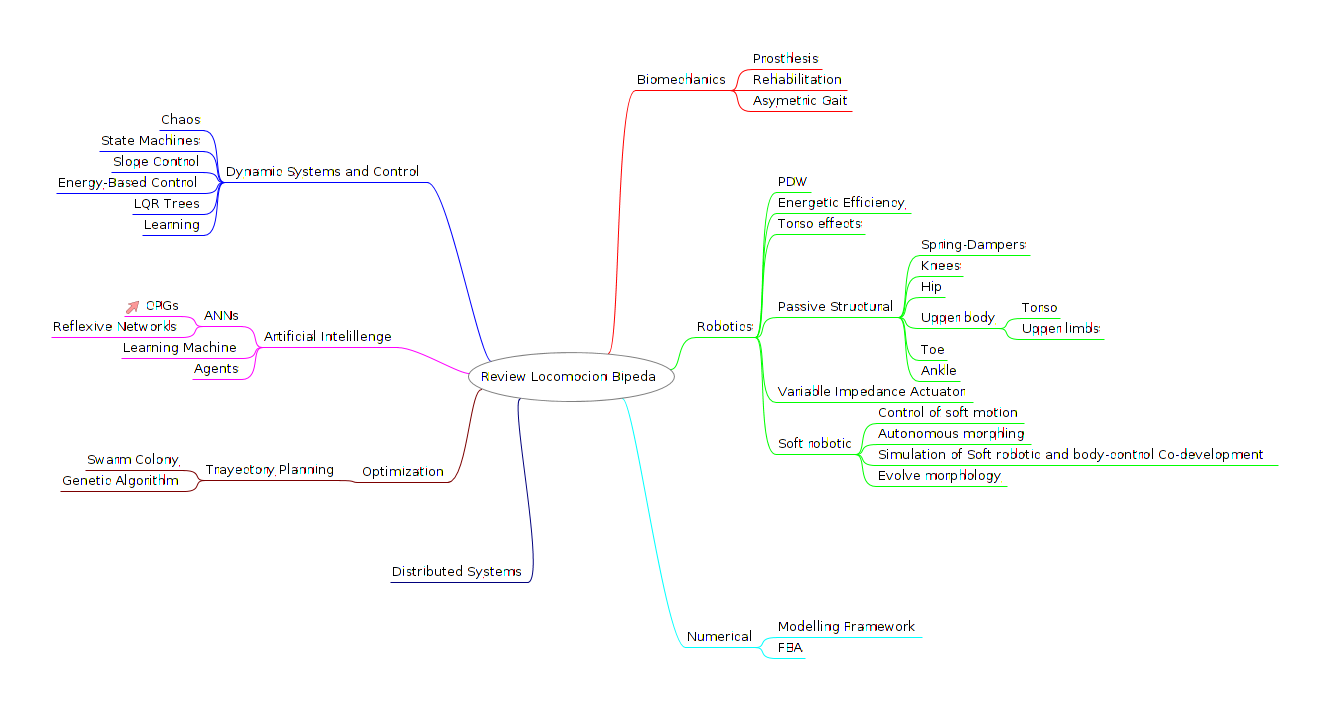
\includegraphics[scale=0.4]{../../images/MindPlaneReviewLocomocionBipeda.png}\\
Las capas y la constituci\'on de cada capa se describen a continuaci\'on,\\
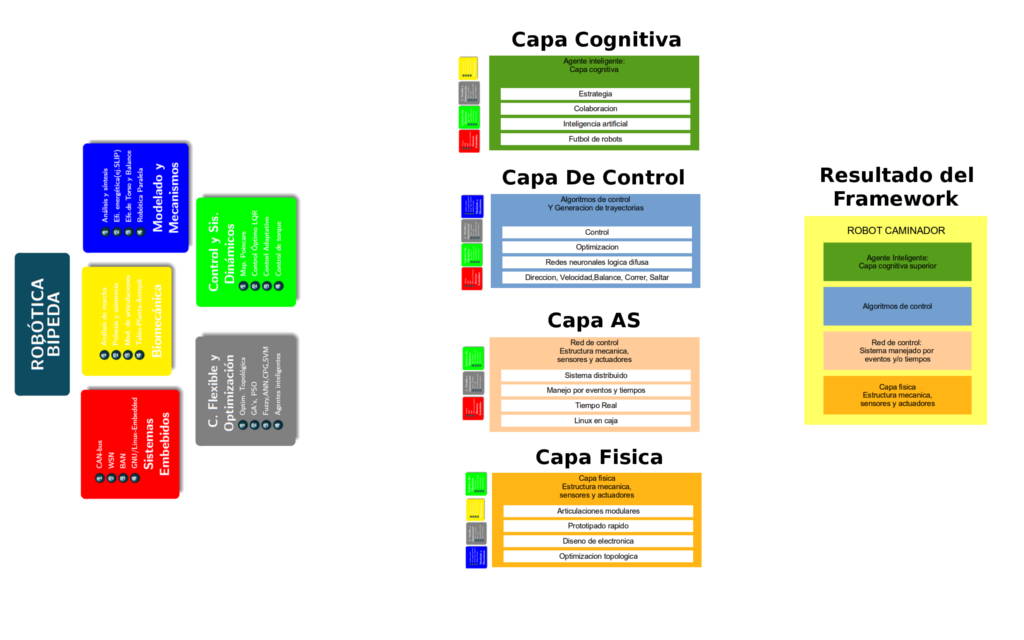
\includegraphics[scale=0.5]{../../images/MakeTheFramework_7.png}\\
\section{Capa morfol\'ogica o mec\'anica}
Esta capa morfol\'ogica se ha centrado mas en el dise\~no mec\'anico y su optimizacion para facilitar el trabajo o estudio de las otras capas del framework. Aqu\'i se hace \'enfasis en: el dise\~no o selecci\'on apropiado de actuadores de inpedancia variable encargados de una mejor relaci\'on con la naturaleza. Los osciladores mec\'anicos que intr\'insecamente generen los ciclos de marcha como en el caso de la din\'amica de la marcha pasiva y las estructuras flexibles. Las herramientas matem\'aticas, los modelos din\'amicos utilizados y las herramientas para la simulaci\'on.
\subsection{Estado del arte}
\subsubsection{Actuadores de Impedancia Variable}
Los actuadores representan los motores de locomoci\'on presentes en las m\'aquinas construidas por el hombre. Al dia de hoy su trabajo industrial estan lejos de la m\'imesis humana. Los actuadores que usa la naturaleza como en el caso de los mam\'iferos son los m\'usculos, estos presentan caracter\'isticas que los motores tradicionales no tienen. Los actuadores de impedancia variable (VIA), por sus siglas en ingles, involucran interacciones con entornos d\'inamicos y desconocidos\cite{Vanderborght2013}. Una breve clasificacion se encuentra en esta \'ultima referencia como: 1) impedancia activa por control, 2) rigidez\footnote{Al referirse a compliance, en el espa\~nol se encaja mejor su opuesto stiffness o constante de rigidez, en los libros de resistencia el opuesto de la nocion de rigidez en la flexibilidad, entonces compliance se ver\'ia como la constante de flexibilidad} y amortiguaci\'on inherente, 3) actuadores inerciales y un combinaci\'on entre los anteriores.\\
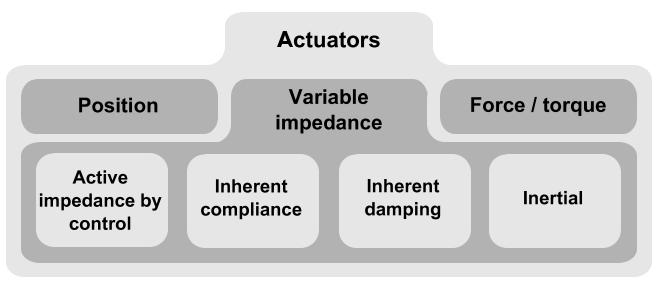
\includegraphics[scale=0.4]{../../images/GeneralClassificationVIAs.png}\cite{Vanderborght2013}\\
La actuaci\'on es la clave de la generaci\'on del movimiento y el control, la carencia de habilidades y el alto costo de los motores actuales ha dificultado el desarrollo de caminadores de alto rendimiento como lo es el uso eficiente de la energ\'ia.\cite{Vanderborght2013}\\
El desempe\~no del control neuronal y m\'ecanico y la funcionalidad de los m\'usculos biol\'ogicos caracterizados por una flexibilidad adaptable o una rigidez variable.\cite{Vanderborght2013,Albu-Schaeffer2009}\\
Algunas limitaciones de los actuadores industriales actuales es que estan dise\~nados para el seguimiento de trayectorias de referencia, lo que idealmente asume una rigidez infinita.\cite{Vanderborght2013}
Las necesidades de actuaci\'on de los retos en locomoci\'on son alcanzados por la tecnolog\'ia de los VIAs como se puede ver en distintos \emph{legged robots}\footnote{Se toma el t\'ermino sin traducir. Robots con patas.}, dispositivos de reabilitaci\'on y pr\'otesis de miembros inferiores.\cite{Vanderborght2013}\\
En los VIAs, el control debe ser optimizado buscando funciones de costo inspiradas biol\'ogicamente. Problemas como la braquistrocroma y generar movimientos Rapidos y flexibles como a su vez riguidos y lentos. Los seres vivos son capaces de variar y planear el cambio de las impedancias de sus cuerpos dependiendo de la actividad que realicen\cite{Albu-Schaeffer2009}.\\
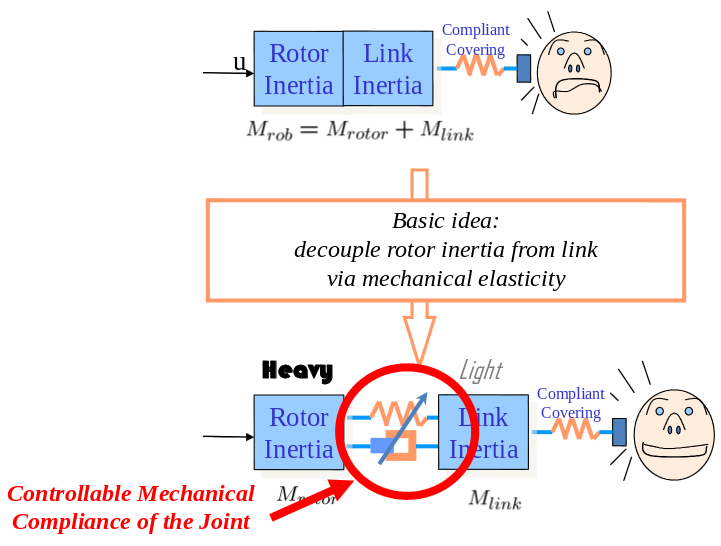
\includegraphics[scale=0.4]{../../images/VIAsConcept.png}\cite{Albu-Schaeffer2009}\\
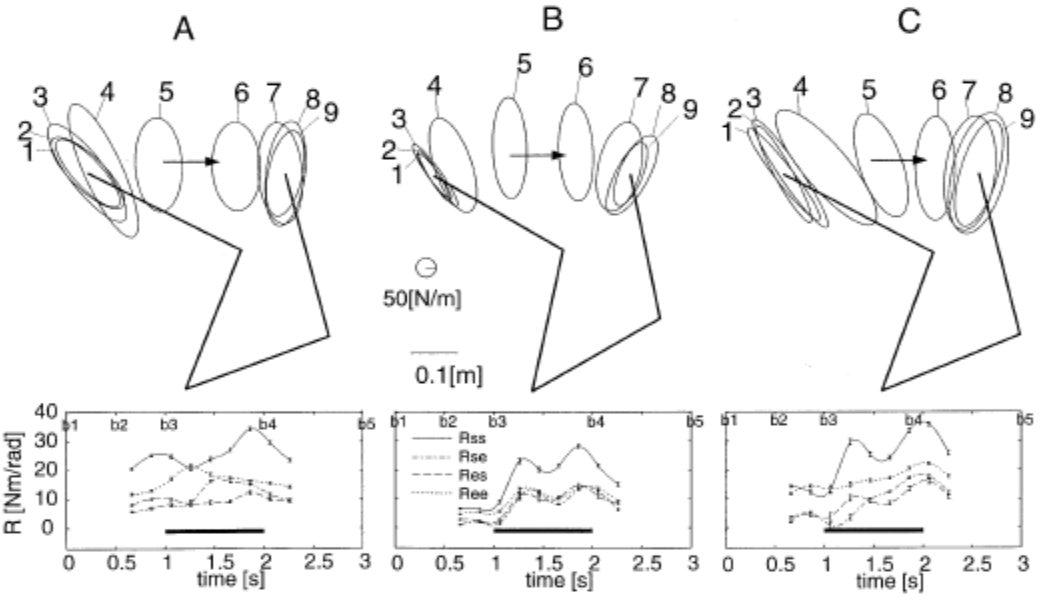
\includegraphics[scale=0.4]{../../images/HumanPlaningImpedance.png}\cite{Albu-Schaeffer2009}\\
Algunas Caracteristicas de los VIA: Un VIA se puede desviar de su posici\'on de referencia que dependiendo de las fuerzas externas y las propiedades mecanicas (principalmente la inercia, la rigidez y la amortiguaci\'on). El punto de equilibrio se define como la posicion en la cual el actuador genera una fuerza nula o \emph{posicion virtual}.\cite{Vanderborght2013}\\
Un caso especial es cuando se propone un caso de impedancia cero, en este punto se logra un actuador que en realidad es una fuente de fuerza. \textcolor{red}{Pregunta: Usando fuentes de fuerza, es posible reducir los efectos de la gravedad que actuan sobre una plataforma robotica b\'ipeda? Como deber\'ia ser el ancho de band de las fuentes?}\\
Los Vias son importates en la Inteligencia Encarnada\footnote{Embodied Intelligence}. Seg\'un Pfeifer y Bongard establecen que un comportamiento adaptativo no est\'a solo el el calculo y el contro, sino que tambien emerge de una interaccion compleja y dinamica entre: la morfolog\'ia del robot, el sistema motosensor y el entorno. Atraves de un dise\~no inteligente del cuerpo y sus actuadores, parte de la inteligencia coputacional puede ser involucrada en la Inteligencia Encarnada logrando que muchas tareas se puedan hacer de formas m\'as sencillas.\textcolor{red}{Pregunta: Lo anterior, puede ser un tema para encontrar un camino de realimentaci\'on para el dise\~no usando las ideas de evolucion?}\cite{Vanderborght2013,Pfeifer2007}\\
\textbf{01 Morphology definition} La morfolog\'ia incluye la forma del cuerpo, las clases de extremidades del cuerpo, la forma en que se interconectan y donde son articulads, las clases de sensores (ojos, oidos, nariz, piel para el tacto y temperatura y el gusto en la boca) y en que parte del cuerpo se encuentran\cite{Pfeifer2007}.\\
\textbf{02 Design bio-optimization} Recordar que la elasticidad del sistema de m\'usculos y tendones, o la deformabilidad de los tejidos en las yemas de los dedos quitan un importante peso de encima en el procesamiento del cerebro.\cite{Pfeifer2007}\\
\textcolor{red}{Idea para CPG y capa electr\'onica.} Comportamientos complicados pueden emerger de reglas simples que corresponden a circuitos neuronales sencillos.\cite{Pfeifer2007}\\
\textcolor{red}{Capa cognitiva.} Por computaci\'on morfol\'ogica, se entiende la libreaci\'on de procesos que el cerebro realiza, para delegarlos a otras partes del cuerpo. Un ejemplo es el hecho de que los musculos de las piernas y los tendones sean el\'asticos de forma que la rodilla, cuando la pierna choca al correr con el piso, realiza peque\~nos movimientos adaptativos sin necesidad del sistema neuronal central de control. El sistema de musculos y tendones por si solo controla la actividad, sistema el cual forma parte de la morfolog\'ia del agente. Relacionado a la marcha, una sola morfolog\'ia puede producir distintos cuencos de atracci\'on correpondientes a diferentes formas de movimiento. Unas mas estables que otras. Cada tipo de marcha tiene su velocidad preferida y optima a la cual moverse.\footnote{basin of attraction}\cite{Pfeifer2007}\\
\textcolor{red}{Capa cognitiva} La robotica evolutiva, se ha utilizado partiendo de un robot con una estructura fija y constate, luego se trata de evolucionar la arquitectura de control lo que generalmente termina en una red neuronal. Por lo general esa evolucion esta aun mas limitada, debido a que la topologia de la red es fija y tampoco evoluciona. Las nuevas tendencias proclaman que el dise\~no ha pasado de moda y ahora lo \emph{in} es la evoluci\'on, esta evolucion es ahora para la morfologia, los materiales y el control.\cite{Pfeifer2007}\\
\textcolor{red}{Capa cognitiva} Morfological evolution, ejemplos de parametros morfol\'ogicos incluyen: longitudes, anchos y alturas de segmentos, el tipo de articulaciones, el tipo de actuadores, la clase de sensores, sus ubicaciones en el cuerpo, las redes neuronales que conectan los sensores y actuadores. \textcolor{red}{Sims} demostr\'o: primero la co-evolucion computacional morfol\'ogica y el control usando \emph{evolved creatures}, segundo nuevas forma de marcha dificiles de imaginar o proponer y tercero se requiere una cantidad enorme de computo. Tarde unas decadas mostrar una creatura construida en la vida real.\cite{Pfeifer2007}\\
Por que el enfoque de control es distinto? Algunas habilidades son requeridas y el control de posicion ya no es eficaz, el control de impedancia y el control de la posicion de equilibrio tienen un mejor desempe\~no en los problemas de locomocion rob\'otica, con un entonrno dinamico y desconocido. Este enfocque permite 1) eficiencia en la generaci\'on de marcha natural, la adaptaci\'on al entorno y protesis de miembros inferiores asi como movimientos explosivos como patear o lanzar, 2) Robustez ante cambios y 3) adaptabilidad.\cite{Vanderborght2013}\\
Algunas definiciones importantes: Impedancia, admitancia, riguidez y flexibilidad. La impedancia mecnica es una relaicon dinamica que se genera entre la fuerza como funcion del tiempo y la el desplazamiento como funci\'on del tiempo. La admitancia es el complemento o lo opuesto de la impedancia. La constaten de riguidez o \emph{stiffness} es la relacion diferencial entre una diferencia infinitesimal de fuerza y posici\'on. La constante de flexibilidad o \emph{compliance} es el inverso. La constante de amortiguaci\'on o \emph{Damping} es la relacion diferencial entre un cambio infinitesimal de fuerza y velocidad, y esta relacionado con la perdida irreversible de la energia mecanica en calor que esta presente en todos los sitemas.\cite{Vanderborght2013}\\
\textcolor{red}{Futuras direccion y objetivos} Los actuadores de impedancia variable estan bajo investigacion para conseguir: seguridad, eficiencia-energ\'etica y movimientos altamente d\'inamicos  para energizar las futuras genraciones de robots, pr\'otesis avanzadas y dispositivos de rehabilitaci\'on\cite{Vanderborght2013}\\
\textcolor{red}{Problemas t\'ecnicos} Hojas tecnicas con especificaciones de los motores son importantes herramientas en el preceso de dise\~no, sin embargo no estan disponibles para los VIA's.\cite{Vanderborght2013}\\
\href{run:/:home/jackmaster/Downloads/[2013 B Vanderborght] Art Variable Impedance Actuators: A review.pdf:pdf}{
\textbf{12: Technical problem}\\
%Datasheets with motor specifications are important tools in the de-sign process, but are yet unavailable for VIA’s.
\textbf{11: Future directions and goals}\\
%Variable Impedance Actuators are under investigation to achieve safe, energy-efficient, and highly dynamic motion for powering the next generation of robots which have to collaborate with humans and interact with an unknown environment. advanced prostheses and rehabilitation devices,
\textbf{10 important descriptions:}\\
%Impedance, admittance, stiffness and compliance Mechanical impedance is a dynamic relation which generates a force (in time) as a function of a displacement (in time). Admittance is the complement of impedance. Stiffness is the differential relation between infinitesimal differ-ences in force and position. Compliance is the inverse. Damping is a dif-ferential relation between infinitesimal changes in force and veloc-ity, and is related to irreversible transduction of mechanical energy to heat and as such takes energy out of the systems.
\textbf{08 About control:}\\ %Why control is seen in a diferent approach? Some required abilities
%Position Control is defeated a better approach is impedace control and equilibrium position contro Position controlis not a properly posed problem controlling the impedance and the equilibrium posi-tion is a well-posed problem that is independent of the knowledge of the environment,an unknown and dynamic environment and the control body-actuator system must have abilities like Efficiency e.g. natural gait generation, adaptation in legged locomotion and prosthetics for lower limbs, explosive motions such as throwing or kicking; Robustness to external perturbations and unpredictable model errors (changes) of the environment, of the robot kinematics Adaptability
\textbf{07 Cognition Layer: evolucion and morphology}\\ % MyQUESTION Could be a subject to find a feedback way to close the general design idea of evolution?
%VIAs are important in Embodied Intelligence. Pfeifer and Bongard [7] state that adaptive behavior is not just control and computation, but it emerges from the complex and dynamic interaction between the robot’s morphology, sensory-motor control, and environment. Through smart design of the body and the actuators, part of the computational intelligence can be outsourced to the embod-ied intelligence making many tasks become simpler.
\textbf{06 VIA's characteristics}\\ %: MyQUESTION Anti-gravity experiment! on force source Why not to build several source forces in a robot to reduce the gravity action? How Bandwith of the force sources should be?}
%A VIA in contrast deviates from its set equilibrium position, depending on the external forces and the mechanical properties of the actuator (mostly iner-tia, stiffness and damping factors). Equilibrium is defined as the position where the actuator generates zero force or torque (also called virtual position by Hogan [5]).
%An extreme case is where the impedance is zero and the actuator forms a force/torque source or transparent actuator, e.g. gravity is a force source.
%Exam-ples where a force/torque source are approached are direct drive motors [6] or constant torque springs.
\textbf{05 Optimal control one way to realize biological characteristics. Some important graphics. A graphic on How humans change/plan thier impedances doing certain tasks?}\\     
%Optimal Control and graphic ideas related to biological inspiration: Soft and fast, stiff and slow => safe brachistochrone
\textbf{04 Applications}\\
%New applications need VIAs technology robots in close human/robot proximity, legged autonomous robots, and rehabilitation devices and prosthe-ses,
\textbf{03 Actual limitation on industrial actuators}\\
%mechanical devices, stiff electrical drives used in industrial robotics, which require accurate, reference-trajectory tracking.
\textbf{02 Biological inspiration}\\
%The functional and neuromechanical control performances of biological musclebe ing the adaptable compliance or variable stiff-ness found in biological systems;
\textbf{01 As an introduction on the subject}\\
%Variable Impedance Actuators (VIA), involving interactions with an unknown and dynamic environment including humans require actuators with dynamics that are not well-achieved by classical stiff actuators. The main classes are active impedance by control, inherent compliance and damping actuators, inertial actuators, and combinations of them, which are then further divided into subclasses. Actuators are key  motion generation and control The lack of suitable actua-tors has hindered the development of high performance machines with capabilities comparable to humans, especially with respect to motion, safety and energy efficiency of human or other animals.
}\cite{Vanderborght2013}\\
El uso de resortes en robots bipedos en las rodillas parece haber comenzado con el Pato y el flamingo del MIT, estructuras saltarinas, que reciclaban la energia de su movimiento. Los SEA usados para control de fuerza y no para almacenamiento de energ\'ia\cite{Grizzle2014}.\\
Hurst dise\~no el modelo plano MABEL y el modelo tridiemensional ATRIAS que incu\'ian resortes largos. En ambos casos los resortes servian para aislar las inercias de los motores de las fuerzas de impacto producidas al tocar el piso y almacenaban la energia de la compresion durante las fases de corrida, cuando la piertna de soporte deba desacelerar disminuyendo el mobimiento del centro de masa del robot. El rbot MABEL ha sido controlado con un grado relativo de dos salidas y lellos han realizado un destacable trabajo de buenos experimentos y el ATRIAS hasta ahora lo ha demostrado\cite{Grizzle2014}.\\
\href{run:/home/jackmaster/Downloads/[2014 Jessy W Grizzle and Christine  Chevallereau and Ryan  W Sinner and Aaron D Ames] Art Survey  paper: Models, feedback control and open problems of 3D bipedal robotic walking.pdf}{
% VIA actuators
%springs into legged robots with revolute knees seems to have started with spring flamingo and spring turkey VIA actuators on hopping robots to recycle energy. series elastic actuator (SEA) designed for force control as opposed to energy storage.\\
%Hurst designed the planar bipedal robot MABEL and the 3D bipedal robot ATRIAS to include large springs, In each case, the springs serve to isolate the reflected rotor inertia of the motors from the impact forces at leg touchdown and to store energy in the compression phase of a running gait, when the support leg must decelerate the downward motion of the robot’s center of mass;\\
%The robot MABEL has been controlled with relative degree 2 outputs and they have performed remarkably well in experiments and ATRIAS has just recently been demonstrated
}\cite{Grizzle2014}
\subsubsection{Din\'amica Pasiva}
La caminata bipeda pasiva surgi\'o de las ideas de los juguetes caminadores del siglo XIX. luego de que en los a\~nos ochenta del siglo XX se analizara la marcha de estos juguetes (McMahon), a finales de dicha decada se desarrollo una serie de caminadores que llamaron la atenci\'on de de la robotica b\'ipeda. McGeer comenzo con una rueda a la cual le retir\'o el rin. Sobre ella analizo los ciclos limite, la zona de atraccion al ciclo limite. Posterior sintentizo la rueda, y removio todos los radios de la rueda excepto dos, los cuales articulo. Concentro la masa en la articulaci\'on. El modelo de dicha rueda sintetizada era modelada por el p\'endulo invertido y el periodo de la marcha es posible de calcular. El siguiente paso de McGeer fue aumentar el radio de los pies y distribuir masas en los pies y la cadera, es un modelo restringido a dos dimenciones, sin embargo las piernas se chocaban con el piso.\\
Goswami estudio el modelo de marcha de compass de McGeer, y encontro que al aumentar las pendientes del piso aparecian bifurcaciones en el modelo din\'amico, lo cual conllevo a aparentes marchas ca\'oticas. Garcia con su modelo simplificado, resalto que usando masas de cadera mucho mayores que las de las piernas, la zona o cuenca de atraccion del ciclo l\'imite aumentaba, a\'un era bastante peque\~no.\\
Wisse utiliz\'o caminadores de piernas rectas con pies planos y resortes en los tobillos y concluyo la similitud con los pies arqueados. En seguida Ikemata utilizo una modificacion en las rodillas y logro una alta estabilidad al conseguir un \'angulo constante en el tal\'on.\\
Narukawa utilizo una configuraci\'on 3D con pasos largos una mayor velocidad sobre otros bipedos construidos con pies arqueados. Nuevamente pie plano y resortes en los tobillos para el yaw y el roll.\\
Los pies arqueados manejan mejor las perturbaciones que los pies puntuales. En 3D a\'un es un reto los movimientos de el roll y el yaw. McGeer no pudo obtener bipedos 3D estables. Los b\'ipedos 3D que han logrado marchas estables se caracterizan por pies grandes. Wisse coloco pies cilindricos y un tobillo que acopla los movimientos de roll y yaw.\\
Colleman y Ruina propusieron un caminador con pies redondos que no tenia equilibrio estatico pero si estabilidad d\'inamica. Para su dise\~no se utilizaron t\'ecnicas de optimizaci\'on pero los parametros obtenidos solo sirvieron en simulaci\'on. Tedrake contruyo el Toddler con pies enomes.\\ 
Collins construyo el mejor 3D conocido al momento, no se uso simulacion es 3D por su complejidad al momento, encontrada en los modelos de colision y fricci\'on. El uso de brazos fue utilizado para contrarestar el Yaw. \\
Narukawa Los pies planos requieren de una articulacion tipo universal o semejante, un material en la planta del pie que evite el deslizamiento. Los resortes en el tobillo son colocados de a pares. Finalmente la estabilidad y oscilaciones del caminador y los pies dependen de la selecci\'on de las constantes de los resortes.\\
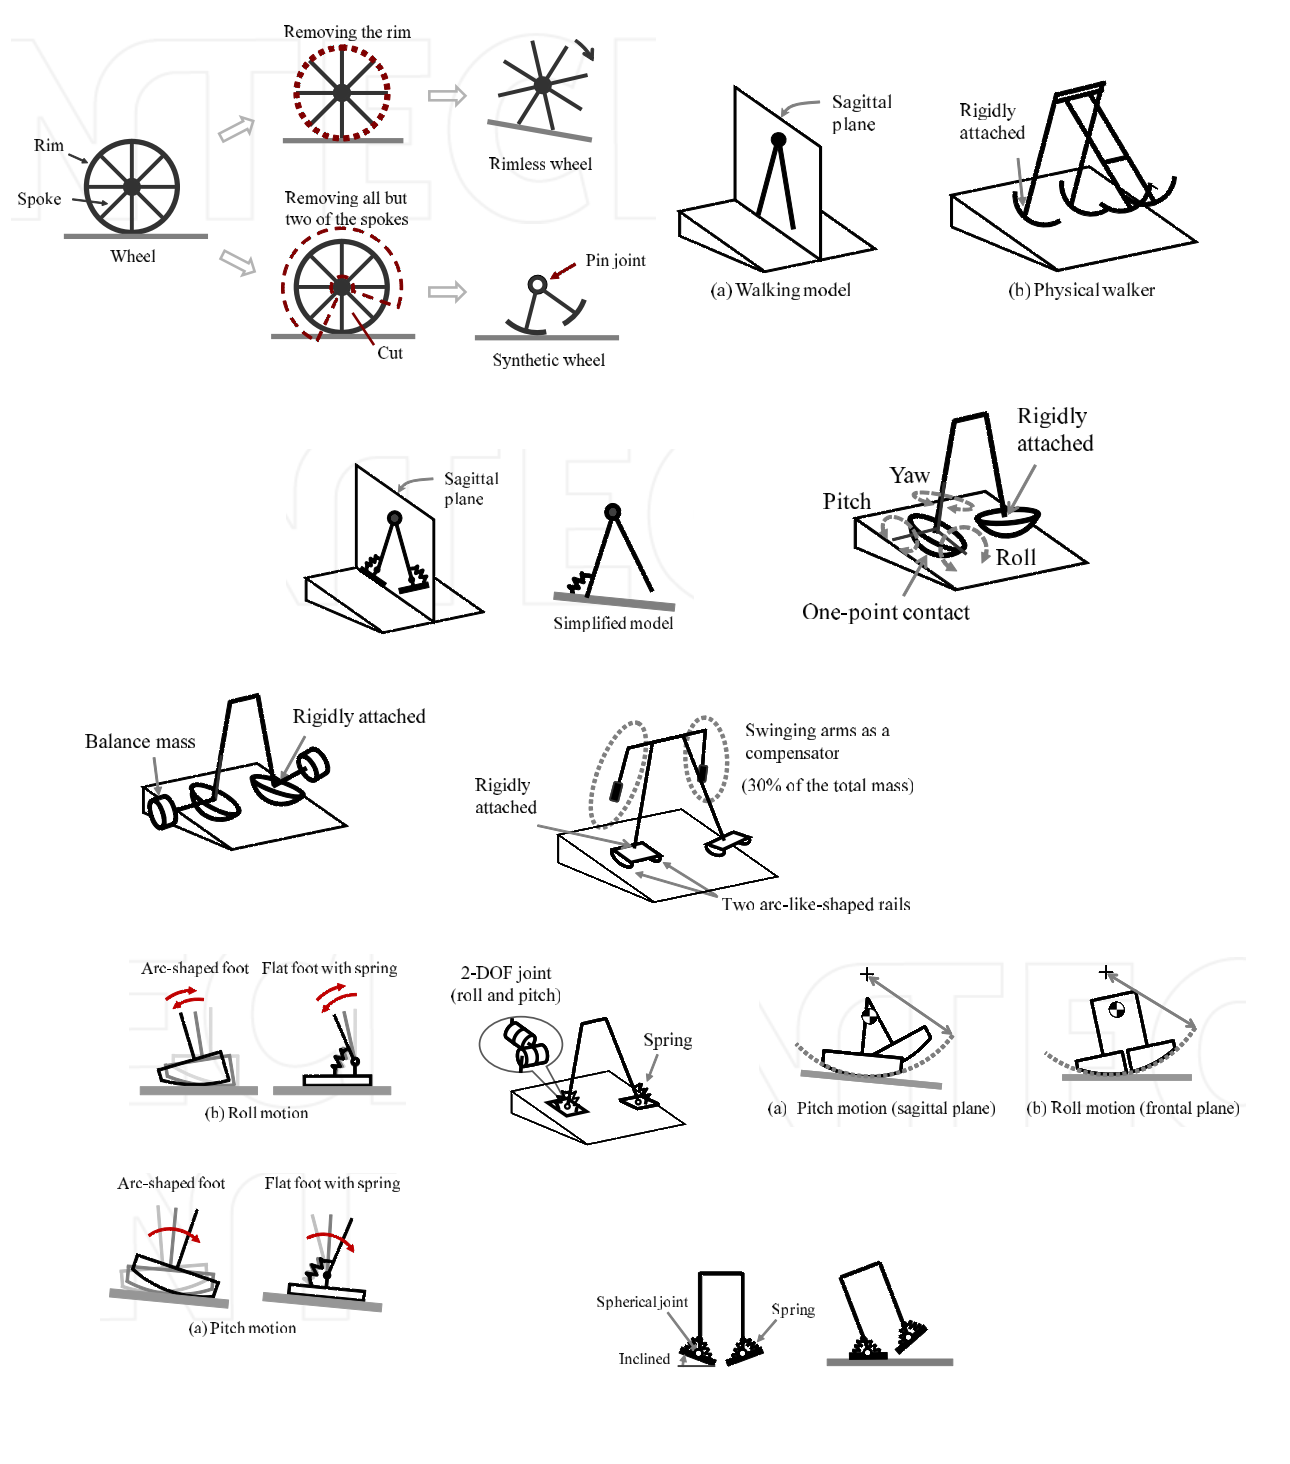
\includegraphics[scale=0.3]{../../images/PWDEvolution.png}\\\cite{Narukawa2010}\\
\href{run:/home/jackmaster/Downloads/Doc Thesis/Walkers/[2010 T Narukawa and K Yokoyama and M Takahashi and K Yoshida] Chp An experimental study of three-dimensional passive dynamic walking with flat feet and ankle springs.pdf}{
%History of PWD evolution\\
%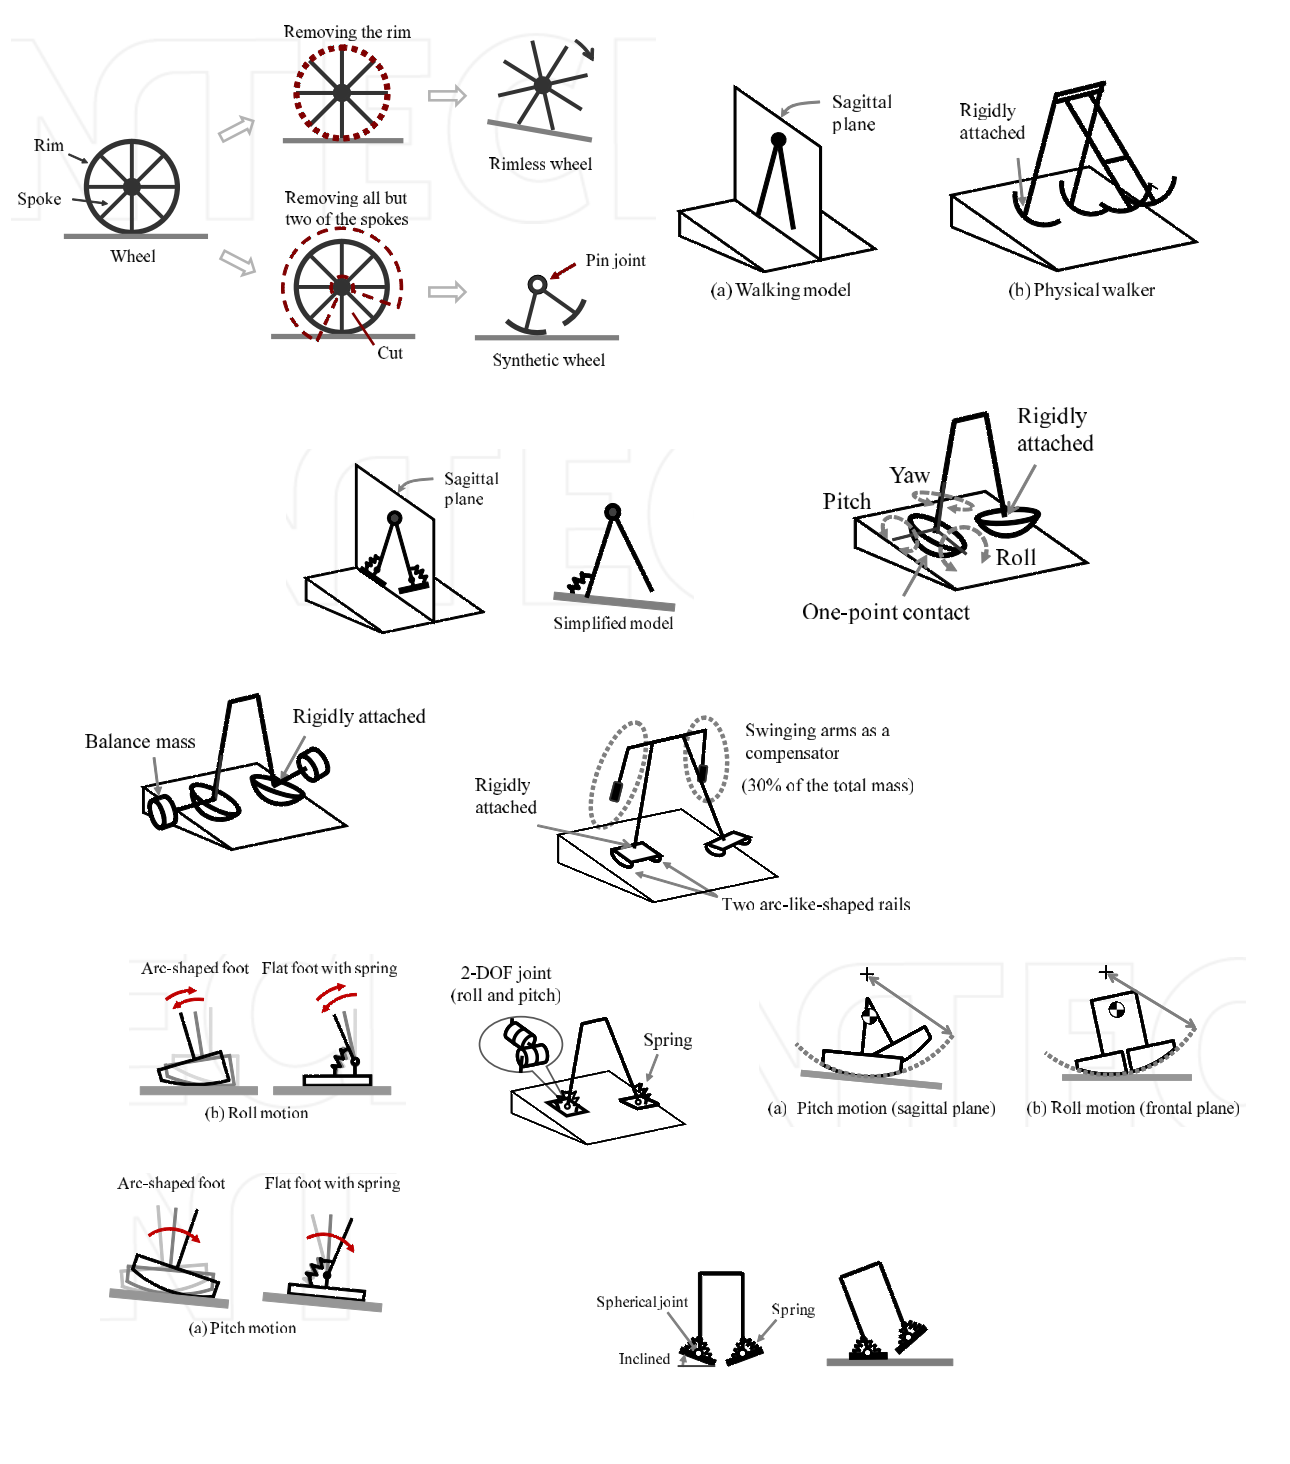
\includegraphics[scale=0.4]{../../images/PWDEvolution.png}
%A rimless wheel can be obtained by simply removing the rim from the wheel, rimless wheel has a periodic motion whose stable region is very large(Wisse\\
%The rim was cut between the spokes, and all but two of the spokes removed. A pin joint and a large point mass were put at the hub, i.e. the hip. If the leg mass is assumed to be negligible compared to the hip mass, the swing leg motion will not disturb the stance leg motion. 
%The step period of the synthetic wheel is determined solely by the free pendulum period of the swing leg.\\
%A kneeless passive biped walker is similar to a synthetic wheel model, however allows for variation of parameters, e.g., radius of the arc feet and lo-cation of the leg mass(McGeer, McGeer’s passive walkers is constrained against falling over sideways, as in numerical simulation models. walkers without knees have a problem of foot scuff-ing at midstance.\\
%Goswami et al. studied the compass model mass is at the hip and legs and the motion is constrained to the sagittal plane. showed that the compass model can exhibit period-doubling bifurcation, eventuallyleading to apparently chaotic gaits, by increasing the slope angle(Goswami. Garcia et al. introduced the simplest walking model, that the leg mass is located at the tip of the leg, and the hip mass is much larger than the foot mass. although the basin of attraction of the simplest walking model is very small. Wisse et al. studied a 2D straight-legged passive walker with flat feet and ankle springs by simplifying the interaction of the spring and the foot. The stance leg with the foot and ankle springs is modeled as a point foot with a torsional spring between the stance leg and the floor. Wisse et al. showed that arc-shaped feet rigidly connected to the legs and flat feet with ankle springs have a similar effect on the disturbance behavior in the simple 2D passive walking model. Ikemata et al. used a stopper to maintain a constant inter-leg angle at heel strike(Ikemata, The stopper enabled the 2D kneed passive walker obtain high stability.\\
%We have developed simple 3D passive walkers that can take longer steps and walk faster than other simple 3D passive walkers with arc-shaped feet. it has flat feet with ankle springs instead of arc-shaped feet rigidly attached to the legs. flat feet with ankle springs stabilize the yaw motion,\\
%arc-shaped feet can handle the dis-turbance behavior of the walkers better than point feet. 3D passive walking remains a challenge because of unstable roll and yaw motions. Roll is rotation about an axis in the direction of motion, and pitch is that about an axis perpendicular to that direction.\\
%McGeer only found unstable motion in 3D passive walking and a physical 3D passive walker was not reported. Stable gaits of the three-dimensional model were found only when the feet were large enough to overlap. Wisse et al. studied a 3D passive walker having cylinder-shaped feet with ankle joints that kinematically couple roll to yaw\\
%Coleman and Ruina built a simple two-leg passive walker with rounded feet attached rigidly to the legs, and laterally extended balance bars as shown. it cannot stand still, it can walk stably in three dimensions. found stable motion of a 3D passive biped using an optimization method to find a set of walker parameters that produced stable walking (Coleman et al., 2001); parameters are far from those of a physical prototype. built by Tedrake et al.(Tedrake et al., 2004; Tedrake, 2004). It has large arc-shaped feet, whose center of the radius of curvature is higher than the center of the total mass, which allows it to stand (Fig. 6). most sophisticated three-dimensional passive walker was built by Collins et al.(Collins et al., 2001) as shown in Fig. 7. 
%did not use simulation studies because numerical simulations of three-dimensional passive walkers are difficult, mainly due to collisions between the swing foot and the ground, and the frictional phenomena between the stance foot and the ground during gaits. reduce the unstable yaw motion, swing arms were attached to the counter side legs.\\
%We investigated simple 3D straight-legged passive walking with flat feet and ankle springs. is composed of a hip, two straight legs, and two feet. The ankles have two degrees of freedom in roll and pitch motion. The main feature the walker to mimic the motion of a 3D straight-legged passive walker with rigidly attachedarc-shaped feet (Tedrake et al., 2004). Kinugasa et al. built a 3D straight-legged passive walker with flat feet and springs attached to ankles; initial spring tension induces an inclined roll angle, but takes only very short steps.\\
%The flat foot and the leg are joined by a universal joint, Sponge sheets are attached to the soles of the feet to increase friction. The torsional spring effect is realized by using a pair of tension springs.\\
%When the spring stiffness is low, oscillating motion is induced by the impact of the feet with the ground. using springs with appropriate torsional spring stiffness effectively reduces the oscillating motion. Appropriate stiffness enables the biped walker to walk smoothly and also stabilizes the walker.
}\cite{Narukawa2010}\\
\cite{Verdaasdonk2009} Verdaasdonk utiliza las caracterizticas de eficiencia de la energia de los caminadores pasivos al ayudarse de las dinamicas de la naturaleza.\\
\href{run:/home/jackmaster/Downloads/Doc Thesis/Walkers/[2009 B W Verdaasdonk and H F J M Koopman and F C T van der Helm] Art Energy efficient walking with central pattern generators: from passive dynamic walking to biologically inspired control.pdf}{
%passive dynamic walking is energy efficient by exploiting the natural dynamics.
}\cite{Verdaasdonk2009}\\
Basado en la dinamica pasiva, se construye un robot de soccer llamado el Stepper-3D, usando una pendiente virtual para emular la cambiata. El dise\~no mecanico esta basado en mecanismos de cuatro barras los cuales mantiene los pies y el tronco orientados paralelos al piso. Se reporta que estos mecanismos ayudan a la estabilidad del robot sin embargo se pierde pasividad. Existe una negociacion entre eficiencia energetica y estabilidad. Tambien se hacen pruebas 3D.\cite{Dong2009}
\subsubsection{Estructuras flexibles}
Plataformas fueron desarrolladas en vestigadas en el contexto de, por ejemplo, apariencias de marcha (similaridad de trayectorias de articulacion durante la locomoci\'on), estabilidad de los patrones de marcha bajo perturbaciones (manteniendo las dinamicas de locomocion sobre terrenos rugosos), la controlabilidad de los patrones de marcha y el posicionamiento de los pies. Un reto primordial en este dominio de investigaci\'on \textcolor{red}{la optimizaci\'on del control en sistema subactuados.} El arqutectura de control requiere de regular las frecuencias de oscilacion de motores de baja potencia para inducir una vibracion libre. Las partes principales del este robot estan compuestas por una viga curva elastica, la forma de la viga se da de forma que pueda genera un movimiento de salto (hopping), el cual es actuado bajo la resonancia del sistema.\cite{Reis2014}\\
El modelamiento de estos robots no es trivial, en este caso la teoria de vigas no puede aproximar de forma apropiada el modelo dinamico de la estructura corporal porque las no-linealidades originadas en las curvatura de la viga y otros enfoques de simulacion numerica como los elementos finitos tradicionales no puden caracterizar de forma efectuva el comportamiento de saltos de la estructura, debido principalmente a los eventos discretos dinamicos como el contacto con el piso y el deslizamiento\cite{Reis2014}\\
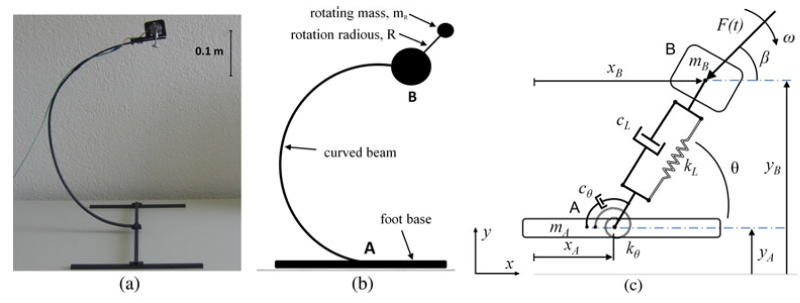
\includegraphics[scale=0.4]{../../images/CurvedBeamIida.png}\cite{Reis2014}\\
\cite{Yu2014}
\subsubsection{Modelos Din\'amicos y Simulaci\'on}
Herramientas para animaci\'on basadas en conceptos puramente cinem\'aticos, trabajan principalmente en grabar o generar de forma manual las trayectorias de las estructuras mec\'anicas. Las herramientas que se basan en leyes f\'isicas y permiten la interaccion con su entorno de forma automatica de forma m\'as acertada, no tiene la necesidad de crear movimientos de datos preescritos. Estas simulaciones basadas en f\'isica han tenidos problemas relacionados a la controlabilidad, la pose de una estructuras basada en fisica es controlada de forma indirecta atraves de fuerzas y torques generados por los actuadores que permanecen en el interior de la estructura. De forma similar a los musculos en los sistemas biologicos. \\
Estas estructuras son subactuadas y solo pueden ser controladas atraves de la manipulacion del contacto externo, dirigiendo el estilo atraves de la aplicacion de fuerzas y torques no es facil, que que su efecto es indirecto y esto puede ocacionar problemas en el equilibrio. Los movimientos obtenidos son precisos y pueden resultar en NO exibir propiedades naturales del mundo real del movimiento, como las marchas simetricas, el uso pasivo de las rodillas o el balanceo de brazos y por lo tanto no pueden ser percibidos como naturales. Estas simulaciones requieren conocimiento de la dinamica multicuerpo de cuerpo riguido, integracion numerica, biomecanica y teoria de optimizacion. Las estrategias de control requieren grandes habilidades y un buen tiempo de ajuste manual de los controladores. Actualmente, los rendimientos en tiempo real en muchas estrategias de control estan limitadas a solo una estructura, para que puedan ser aprovechadas por las arquitecturas de los computadores actuales\cite{Geijtenbeek2012}\\
\href{run:/home/jackmaster/Downloads/[2012 T Geijtenbeek and N Pronost] Art Interactive Character Animation Using Simulated Physics:
A State-of-the-Art Review.pdf}{
%Kinematics-based animation frameworks rely heavily on existing motion data, either recorded or manually crafted through keyframing.\\
%physics-based characters and objects automatically interact in a way that is physically ac- curate,without the need for additional motion data or scripts.\\
%physics-based characters have several issues related to controllability (or lack thereof), the pose of a physics-based character is controlled indirectly, through forces and torques generated by actuators that reside inside the character—similar to muscles in biological systems.\\
%physics-based character are unactuated and can only be controlled through deliberate manipulation of external contacts.\\
%Directing style through applica-tion of forces and torques is non-trivial, since their effect is indirect and may disrupt basic tasks such as balance.\\
%their motions are physically accurate, they may not exhibit natu-ral properties of real-world motion, such as gait symmetry, passive knee usage or passive arm swing [BSH99, Nov98,dLMH10], and may therefore not be perceived as natural.\\
%physics-based characters are less reactive during direct control tasks than kinematics-based characters.\\
%physics-based requires at least some knowledge of multi-body dynamics, numerical integration, biomechan-ics and optimization theory. control strategies require skilful and time consuming manual tuning. Currently, real-time performance of many recent control strategies (e.g.[dLMH10, JL11b]) is still limited to around a single character at a time on modern hardware.\\
}\cite{Geijtenbeek2012}\\
Por lo general los motores de simulaci\'on basados en f\'isica estan construidos por:\\
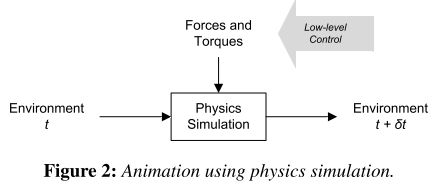
\includegraphics[scale=0.4]{../../images/PhysicsSimulation.png}
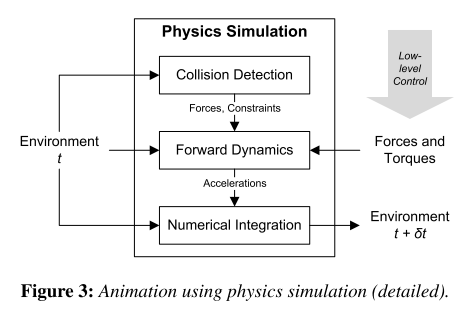
\includegraphics[scale=0.4]{../../images/PhysicsSimulationDetailed.png}\cite{Geijtenbeek2011}\\
Dos formas son usadas para las \emph{colisiones}: por penalizacion de fuerzas y por restriciones de colisi\'on. Las fuerzas de friccion, usando el cono de friccion de Coulomb. La frici\'on din\'amica o deslizamiento puede ocurrir cuando una colision responde a una fuerza que permanece por fuera del cono. Al modelar por restricciones, una articulacion simbolica es construida sobre el punto de colision que restringe el movimiento de los objetos en contacto. La forma en que la fricion es modelada puede tener un impacto significante en las estrategias de control de movimiento subsecuentes.\cite{Geijtenbeek2011}\\
La \emph{din\'amica directa} es calculada para las aceleraciones angulares y lineales de los objetos simulados, basados en fuerzas externas y restriciones. La \emph{din\'amica indirecta} es calcular los torques y las fuerzas requeridas para que una estructura logre un movimiento especifico. Este proceso es usado frecuentemente en biomecanica para analizar el movimiento de los humanos. Tambien esposible utilzar una combinacion de dinamicas directa e inversa. En este caso, es posible controlar una parte de los movimientos cinematicamente y la otra para calcular la parte calcular las cargas para realizar un determiado movimiento esta situacion es conocida tambien como dinamica mixta
\href{run:/home/jackmaster/Downloads/[2011 T Geijtenbeek and N Pronost and A Egges and M H Overmars] Art Interactive Character Animation using Simulated Physics.pdf}{
%two ways to respond to collisions: a penalty force, collision constraint.\\
%Coulomb friction cone. Dynamic friction (sliding) will occur when a required collision response force lies outside this cone.\\
%modeled through constraints, a symbolic link is constructed at the point of collision that restricts movement of the colliding objects\\
%The way in which friction is modeled can have a signifi-cant impact on subsequent motion control strategies.\\
%Forward dynamics is to compute linear and an-gular accelerations of simulated objects, based on external forces and constraints.\\
%Inverse Dynamics compute the torques and forces required for a character to perform a specific motion. This process is used frequently in biomechanics to an-alyze the motion of humans. It is also possible to combine forward and inverse dynamics. For instance, it is possible to control one half of a virtual character kinematically, use inverse dynamics to compute torques required to perform that motion, and perform forward dynamics to compute the motion of the other half, as mixed dynam-ics.\\
}\cite{Geijtenbeek2011}\\
Los m\'etodos de s\'intesis de marcha son apliamente divididos dentro de cinco categorias 1) Modelos de pendulo invertido, 2) modelos de caminata pasiva, 3) metodos de ZMP, 4) m\'etodos de optimizaci\'on y 5) m\'etodos basados en control. De estos grupos nuevamente se reagrupan en dos grandes grupos 1) los que ofrecen una soluci\'on en tiempo real para la planeacion de caminata. 2) los metods basados en optimizaci\'on y an\'alisis usando modelos esquel\'eticos o musculo-esquel\'eticos con muchos grados de libertad.\cite{Xiang2010}\\
Los metodos basados en optimizaci\'on pueden obener medidas del desempe\~no humano de forma simultanea. Estos metodos porducen soluciones otimas y perfiles de fuerzas articulares sugetas a todas las retricciones necesarias.\cite{Xiang2010}\\
Modelos de marcha:\\
Modelos de aproximaci\'on mecanica: la literatura esta generalmente simplificada de dos formas 1) aproximacion mecanica y 2) simplificacion del movimiento de la marcha. Para los modelos basados en el esqueleto, los musculos agrupados en las articulaciones son agrupados y representan un torque en la union. Por lo tanto, los modelos esqueleticos son comunmente usados en la simulacion del movimiento humano debido a su simplicidad y eficiencia computacional. En contraste con los sistemas musculo-esqueleticos que apuntan a la prediccion del movimiento y las fuerzas al niverl muscular. Este ultimo es crucial para estudios fisiol\'ogicos y depnde de nuestro entendimiento en la forma de excitaci\'on de los m\'usculos y las estrategias de reclutamiento muscular durante el movimiento de la marcha.\cite{Xiang2010}\\
Simplificacion del movimiento de la marcha: Estudios experimentales, la complejidad del movimiento incluye siete fases para una marcha completa. Una marcha simplificada ha sido ampliamente dividida en cuatro categorias: 1) movimiento con suporte y balanceo simple, 2) soporte simple con soporte doble instant\'aneo, 3) sporte simple y doble para un paso y 4) marcha completa en cada zancada.\cite{Xiang2010}\\
\href{run:/home/jackmaster/Downloads/Doc Thesis/Walkers/+[2010 Y Xiang and J S  Arora and K Abdel-Malek] Art Physics-based modeling and simulation of human walking: a review of optimization -based and other approches.pdf}{
%The gait synthesis methods are broadly divided into five categories: (1) inverted pendulum model; (2) passive dynamics walking; (3) zero moment point (ZMP) methods; (4) optimization-based methods; and (5) control-based methods.\\
%the paper is divided into two parts. (1) simple gait models and real-time walking plan-ning. (2)optimization-based methods for gait simulation and analyses using skeletal or muscu-loskeletal models with many degrees of freedom.\\
%And for (2), optimization-based approach for synthesizing natural and smooth human walking, optimal control methods for walking simulation\\
%The method can optimize any human-related performance measure simultaneously. the method produces optimal motions and joint force profiles subjected to all the necessary constraints\\
%Gait modeling\\
%Mechanical model approximation\\
%the literature are generally simplified mainly in two ways: (1) mechanical model approximation, and (2) gait motion simplification.\\
%For a skeletal model, the muscle group at a joint is lumped and represented by a joint torque. Therefore, skeletal models are commonly used in human walking simulation due to their simplicity and computational efficiency. In contrast, the musculoskeletal model aims to predict the motion and forces at the mus-cle level. This is crucial for physiological studies, and it deepens our understanding of muscle excitation and recruit-ment strategies during the walking motion.
%Gait motion simplification\\
%experimental study, the complex walking motion includes seven phases in a complete gait cycle. a simplified gait cycle has been broadly divided into four categories: (1) single support swing motion; (2) single support with instantaneous double support; (3) single support and double support—a step; (4) complete gait cycle—a stride.\\
}\cite{Xiang2010}\\
Durante la fase de soporte la pierna de apoyo actua como un pendulo invertido sin nada de masa mas que en la parte superior, porlotanto la caminta humana es vista como una oscilacion respesto a un punto est\'aticamente inestable. Como la marcha humana puede ser dinamicamente estables, robusta y con eficiencia energetica al mismo tiempo? La marcha humana muestra que la mayoria de los musculos estan altamente activos solo al comienzo y final de las fases de apoyo y balanceo\cite{Verdaasdonk2009}.\\
\href{run:/home/jackmaster/Downloads/Doc Thesis/Walkers/[2009 B W Verdaasdonk and H F J M Koopman and F C T van der Helm] Art Energy efficient walking with central pattern generators: from passive dynamic walking to biologically inspired control.pdf}{
%During the stance phase, the stance leg acts as an inverted pendulum with a mass on top. Therefore, human walking is statically unstable.\\
%how ‘human gait’ can be dynamically stable, robust and energy efficient at the same time.\\
%human walking show that most of the muscles are only highly active at the beginning and end of the stance and swing phase\\
}\cite{Verdaasdonk2009}\\
Modelo de caminador:\\
Un pue permanece plano contral el piso sin deslizarse solo cuando la reaccion de fuerzas y torques sobre la interface satisfaces las inequaciones estrictas; en particular cuando la componente normal de la fuerza de reaccion de piso GRF es positiva, ya que el piso no puede atraer contra si mismo como si lo haria una unios con tornillos en un manipulador industrial. Ademas las fuerzas tangenciales deben de quedar dentro del cono de fricci\'on, por lo tanto el contacto entre el robot y su entorno (el piso) es una reaccion unilateral e intermitente. La fuerza debe ser positiva o cero desde que el piso pueda presionarse, sin embargo no puede jalar sobre el robot. Una restricci\'on adicional para evitar o permitir el deslizamiento debe ser planteada\cite{Grizzle2014}.\\
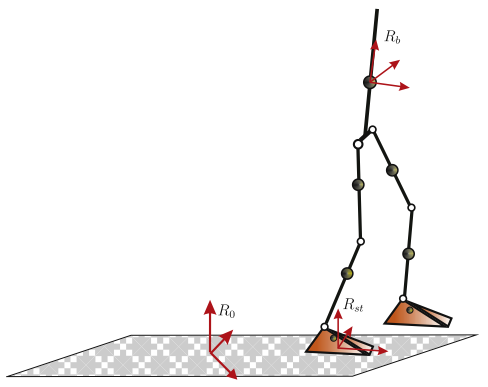
\includegraphics[scale=0.4]{../../images/GeneralBipedModel.png}\cite{Grizzle2014}\\
Para los propositos de dise\~no del control, una version actuada de un modelo hibrido multifase en 4) es usad deonde cada fase corresponde a una especifica compbinacion de condiciones complementarias siendo tambien cero o no cero. Enumearndo estas restriciones se llega a una forma natural de estructurar la caminata a partir de un grafo dirigido, para entonces motivar la aplicacion de la teoria de sistemas hibridos\cite{Grizzle2014}.\\
El robot de por si es modelado cl\'asicamente por una estructura compuesta por eslabones r\'igidos. Cuando el contacto ocurre entre el pie y el piso, este es asumido como un contacto r\'igido. Con estas suposiciones, una forma de obtener un modelo de varias fases de caminata es primero construir una base foltatne de un modelo Lagrangiano del robot (sin asumir las condiciones de contacto), y entonces a\~nadir las fuerzas de contacto por medio del principio de D'Alambert.\cite{Grizzle2014}\\
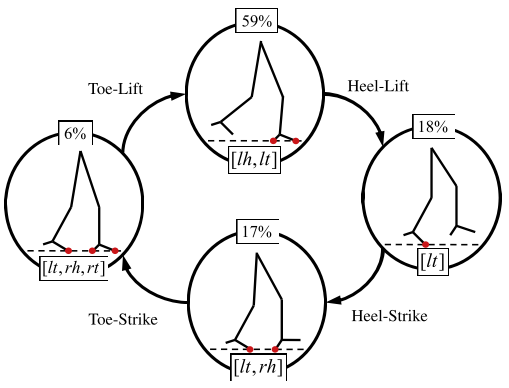
\includegraphics[scale=0.4]{../../images/DirectedGraphBipedModel.png}\cite{Grizzle2014}\\
Modelos simples:\\
Cuatro modelos de baja dimension que son frecuentemente usados como aproximaci\'on de los robots camiadores. De izquierda a derecha: el modelo lineal de pendulo invertido (LIPM) agrupa las masa de el robot en un punto que se mueve a altura constante y asume las piernas sin masa; el pendulo invertido con volante IPF relaja la suposici\'on de la altura constante y a\~nade un volante para que tome en cuenta el momento angular interno; el modelo de resorte cargado de pendulo invertido (SLIP) a\~nade un modelo de resorte a las piernas sin masa del robot; y el modelo de comp\'as trata el robot como un pendulo doble con masa agrupadas sobre las piernas de soporte y balance.\cite{Grizzle2014}\\
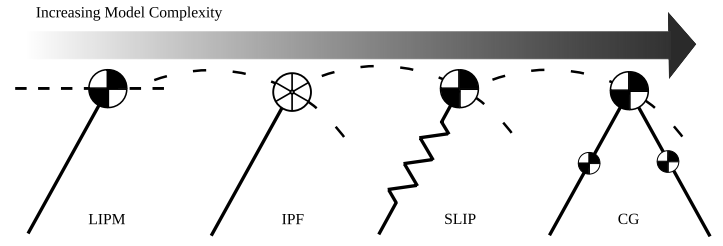
\includegraphics[scale=0.4]{../../images/SimpleBipedModels.png}\cite{Grizzle2014}\\
un enfoque que logra la estabilidad asimt\'otica de la locomoci\'on bipeda en la presencia de la subactuaci\'on, las condiciones de contacto entre el robot y el piso son extremadamente importantes para el control de un b\'ipedo\cite{Grizzle2014}.\\
\href{run:/home/jackmaster/Downloads/[2014 Jessy W Grizzle and Christine  Chevallereau and Ryan  W Sinner and Aaron D Ames] Art Survey  paper: Models, feedback control and open problems of 3D bipedal robotic walking.pdf}{
% Model Walker\\
%A foot remains flat on the ground without slipping onlywhenthe reaction forces and torques at the interface satisfy strict inequalities; in particular, the normal component of the ground reaction force must be positive, as the ground cannot ‘‘pull’’ against a foot as a bolt will for a manipulator; in addition, tangential forces must lie in a friction cone.\\
%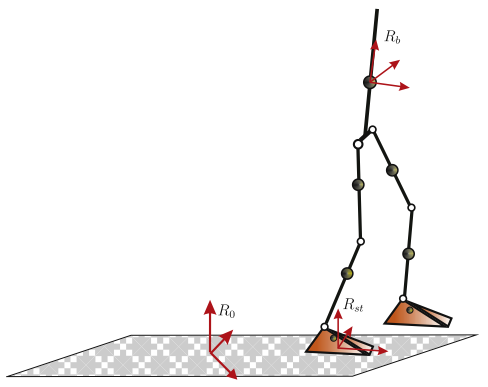
\includegraphics[scale=0.4]{../../images/GeneralBipedModel.png}\\
%contact between the robot and its environment (the ground) is unilateral and intermittent.\\
%force must be positive or zero since the ground can push, but cannot pull, on the robot. Additional con-straints to avoid (or to allow) slipping also exist.\\
%For the purposes of control design, an actuated version of the multi-phase hybrid models in (4) are used,whereeach phase corresponds to a specific combination of complementarity conditions being either zero or non-zero. Enumerating these constraints leads to a natural way of structuring a walking gait as a directed graph, thereby motivating the application of hybrid sys-tems theory.\\
%The robot itself is classically modeled as a tree structure composed of rigid links. When contact occurs between the feet and the ground, it is assumed to be a rigid contact. With these assumptions, one way to obtain a model for the various phases of a walking gait is to first construct a floating-base Lagrangian model of the robot (i.e., no assumptions on ground contact), and then add in ground contact forces via D’Alembert’s principle.\\
%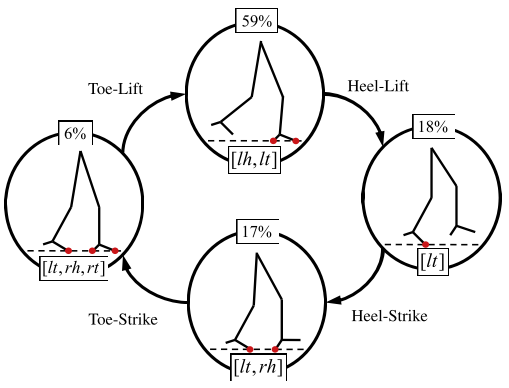
\includegraphics[scale=0.4]{../../images/DirectedGraphBipedModel.png}\\
%Simple models\\
%Four low-dimensional models that are frequently used as approximate representations of walking robots. From left to right: the Linear Inverted Pendulum Model (LIPM) lumps the mass of the robot at a point moving at a constant height and assumes massless legs; the Inverted Pendulum with Flywheel (IPF) relaxes the assumption on constant height and adds a flywheel to account for internal angular momentum; the Spring-Loaded Inverted Pendulum(SLIP) adds a spring to model a robot’s legs as a massless pogo stick; and the Compass-Gait Biped (CG) treats a robot as a double pendulum with lumped masses on the stance and swing legs.\\
%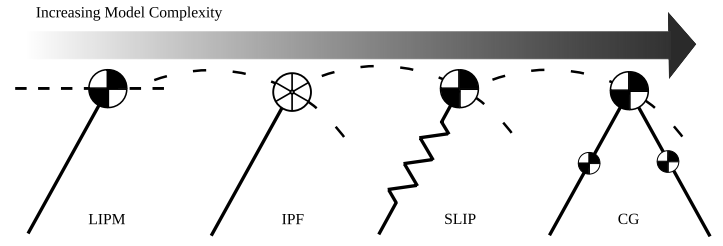
\includegraphics[scale=0.4]{../../images/SimpleBipedModels.png}\\
%an approach to achieving asymptotically stable bipedal locomotion in the presence of underactuation. the contact conditions between the robot and the ground are extremely important for the control of a biped.
}\cite{Grizzle2014}\\
Resultados de simulaciones, sobre HOAP y DARwIn-OP en el software de Webots muestra la adecuacion del sistema locomotor basado en CPGs para generar caminata bipeda sobre diferentes robots.\cite{Matos2014}
\subsection{Futuras tendencias}
\subsubsection{Selecci\'on y/o dise\~no de actuadores}
Un prototipo de un actuador de riguidez variable (VSA-Cube) basado en el modelo bidireccional agonista-antagonista, pensando en bajos costos. Se presenta de forma Open-Source y DIY, el mecanismo VSA-Cube con electronica embebida y conexiones mecanicas y electricas. Es un servo, con sensores de posicion, tarjetas electronicas y algoritmos de control del eje de salida, comunicacion con bus I$^2$C permite diversas configuraciones modulares, entre ellas caminadores b\'ipedos. Se propone una ficha tecnica aunque sujeta algunos problemas de parametros. Ademas de esto es presentado un modelo dinamico para su an\'alisis.\cite{Catalano2011}
Aun cuando, en la mayoria de los estudios sobre caminata dinamica, la rigidez (o \emph{compliance}) es cambiada off-line. La transicion de diferentes patrones, velocidades y largo de paso atraves del cambio de rigidez en tiempo real no ha sido investigado. El concepto de \emph{Caminata Pasiva Controlada}. Los efectos de torque articular y la riguidez articular sobre el desempe\~no al caminar, control de velocidad, transicion de patrones de marcha fueron estudiados, usando CPGs sobre una plataforma con extremidades superiores, pie plano y articulaciones con riguidez adaptable.\cite{Huang2014}\\
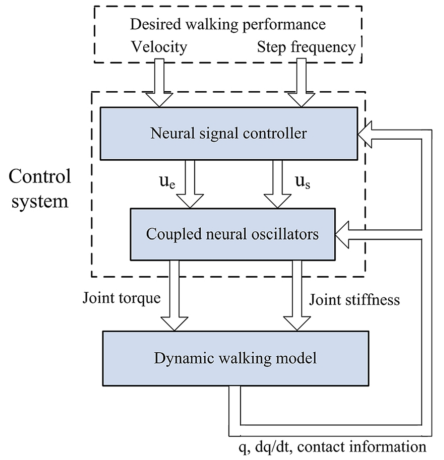
\includegraphics[scale=0.4]{../../images/CPG-PWD-VIA.png}\cite{Huang2014}
\subsubsection{Almacenamiento y reciclado de la energ\'ia de impacto}
\subsubsection{Dise\~no morfol\'ogico}
Osciladores mecanicos acoplados con CPGs. Intestigacion en co-evoluci\'on.\cite{Verdaasdonk2009}\\
\href{run:/home/jackmaster/Downloads/Doc Thesis/Walkers/[2009 B W Verdaasdonk and H F J M Koopman and F C T van der Helm] Art Energy efficient walking with central pattern generators: from passive dynamic walking to biologically inspired control.pdf}{
%Mechanical oscillator coupled with CPG's. Co-evolution research.
}\cite{Verdaasdonk2009}\\
Materiales y morfolog\'ias no convencionales en sistemas roboticos, buscando las ventajas de las propiedaes mecanicas (como lo son la forma, elasticidad, viscosidad, flexibilidad, densidad, pegajosidad) son cruciales en las investigaciones de la Inteligencia Encarnada. Las interaccion entre sistemas fisicos y sus alrededores, son de particular importancia en el desarrollo de tecnologia y nuevos comportamientos adaptativos. Los sistemas biologicos usalmente la circuiteria neuronal se adapta continuamente a los dramaticos cambios de las estructuras. Materiales flexibles como polimeros son examinados como una novedosa forma de sensores y actuadores.\cite{Iida2011}\\
El control de movimentos flexibles, exhibe controles de movimiento mas dinamicos y energeticamente eficientes. Se requiere dise\~nos de cuerpo entero usando materiales flexibles y deformables. Las dimensiones de los parametros de dise\~no estan cambiando dramaticamente dependiendo a su vez de la postura que tome el cuerpo.\\
Hacia una morfologia autonoma, cambios plasticos y el crecimiento de los cuerpos estructurales. La modularidad y la conectividad son la clave para los cambios plasticos en la morfologia de los robots. Algunas cuestiones mofologicas se plantean: Como podemos construir mecanismos de coneccion mas flexibles sobre cada modulo, tal como una celula puede conectarse con otros modulos? Como pueden estos modulos variar sus propiedades mecanicas (m\'as elasticos, m\'as rigidos, m\'as flexibles)? Como se pueden autorreparar? Como pueden replicarse para el cresimiento fisico?\cite{Iida2011}\\
Se requiere herramientas de simulacion y modelado para un desarrollo sistematico en este campo de investigacion. Es necesario simular mas modelos continuos en adicion con los discretos que representan eslabones y articulaciones mecanicas. La robotica flexible usa controles decentralizados. Simular cambios morfologicos y de propiedades materiales son retos actuales. Que relaciones existen entre morfologias y funcionalidades: auto-organizacion, auto-estabilidad y auto-ensamble. Se cree que estos desarrollos traeran un alto impacto en el desarrollo de protesis y elementos de rehabilitaci\'on.\cite{Iida2011}\\
\subsubsection{Modelado y simulaci\'on}
Investigadores estan desarrollando modelos de caminata humana en tiempo real teniendo una alta fidelidad y obtebiendo un control online, biomecanica cl\'inica y estudios de patolog\'ias en la marcha. En a\~nos recientes ha existido mucho progreso en la simulaci\'on de caminata humana, especialmente utilizando las tecnicas dee optimizacion de modelos de gran escala. Los modelos de varios grados de libertad (DOF) pueden ser considerados, y mas variables de dise\~no pueden ser incluidas en la formulacion de optimizacion tal que una caminata humana mas natural puede ser obtenida.\cite{Xiang2010}\\
La simulaici\'on de caminata se desarrolla en dos campos:
En el campo de la robotica, el control en tiempo real de caminata bipeda esta principalmente orientada, y modelos simplificados de caminata, tal como el modelo de pendulo invertido y la caminata dinamica pasiva, son usados para este proposito.\\
En el campo de la Biomec\'anica, el analisis de la marcha es usado sobre un modelo musculo-esqueletico que puede dar un mayor detalle acerca de la fisiologia de la marcha humana. Varios investigadores, desarrollaron marcos de optimizacion para simular la marcha de un paso, los cuales consideran el soporte simple y doble de las fases.\cite{Xiang2010}\\
Ecuaciones de movimiento y analisis de sensibilidad\\
Ecuaciones de movimiento\\
Un modelo plano de pocos eslabones, governado de ecuaciones puede ser escrito en una forma matricial tal que el calcuo es bastante sencillo y eficiente.\\
Para modelos espaciales, la ecuaciones de movimiento necesitan ser derivadas en una forma mas sistematica. En este proceso, el metodo de Denavit-Hartenverg, el metodo recursivo de Newton-Euler, y los metodos recursivos de Lagrange son usalmente usados para formular la cinematica y dinamica de los modelos espaciales.\\
Los modelos musculo-esqueleticos son governados por ecuaciones que pueden ser genradas por un software comercial de dinamica multicuerpo como ADAMS, VirtualLAB, SD/FAST.\cite{Xiang2010}\\
\href{run:/home/jackmaster/Downloads/Doc Thesis/Walkers/+[2010 Y Xiang and J S  Arora and K Abdel-Malek] Art Physics-based modeling and simulation of human walking: a review of optimization -based and other approches.pdf}{
%Researchers are developing real-time human walking models having high fidelity aimed at online control, clinical biomechanics, and pathological gait studies.\\
%In recent years, there has been much progress in research on simula-tion of human walking, especially in utilizing optimization techniques for large-scale models. Models with large degrees of freedom (DOF) can be considered, and more design vari-ables can be included in the optimization formulation so that more natural human walking simulation can be achieved.\\
%walking simulation in two research fields:
%robotics field, real-time control of biped walking is the main focus, and simplified walking models, such as the inverted pendulum model and passive dynamicswalking, are usually used for this purpose.\\
%biomechanics-based gait anal-ysis using a musculoskeletal model can give more details about the physiology of human walking.\\
%Anderson and Pandy (2001a), Xiang et al. (2009b), and Mu and Wu (2003) developed the opti-mization framework to simulate one-step walking, which consisted of single support and double support phases.\\
%Equations of motion and sensitivity analysis\\
%Equations of motion\\
%planar human model with a few linkages, the governing equations can be written in a simple matrix form so that the calculation is quite straightforward and efficient\\
%for a spatial model, the equa-tions of motion need to be derived in a more systematic way. In this process, the Denavit–Hartenberg (DH) method (Denavit andHartenberg 1955), the recursiveNewton–Euler method, and the recursive Lagrangian method are usually used to formulate kinematics and dynamics for the spatial models\\
%musculoskeletal model, the govern-ing equations can be generated by commercial multi-body dynamics software such as ADAMSTM, VirtualLabTM,and SD/FASTTM (Anderson and Pandy 2001a).\\
}\cite{Xiang2010}\\
Analisis de sensibilidad:\\
Recientemente, una planeaci\'on del movimiento dinamico fuer resuelta usando gradientes analiticos in el proceso de optimizacion para mejorar la eficiencia computacional. Lo et al. (2002) presentaron un marco general de prediccion del movimiento humano incorporando las ecuaciones inversas recursivas de Newton-Euler con gradientes analiticos usando algebra de Lie.\cite{Xiang2010}\\
Las ecuaciones de Newton-Euler para sistemas con topologias de arbol o ramificadas. Entonces los algoritmos son aplicados para la planeadion del moviento dinamico para le dise\~no de las marchas roboticas de rehabilitaci\'on.\cite{Xiang2010}\\
Dinamica directa, dinamica inversa y dinamica predictiva:\\
La dinamica directa calcula el movimiento dado por las fuerzas mediante la integracion de las ecuaciones de movimiento con condiciones inciales especificadas. En contraste la dinamica inversa calcula el movimiento asociado a la fuerzas que lideran un movimiento preescrito para el sistema. La optimizacion con dinamica directa,toma las fuerzas como las variables de dise\~no en el problema de optimizacion. La marcha optima es determinada por la minimizacion de las medidas de desempe\~no humano sujetas a las restriciones fisicas. Para la optimizacion con dinamica inversa las variables de dise\~no son las perfiles angulares de las articulaciones. Una iteracion de optimizacion, toma las fuerzas directamente calculadas de las ecuaciones de movimiento tal que la integracions numerica no es necesaria. El problema de optimizacion es resuelto para la marcha de movimiento \'optima.\cite{Xiang2010}\\
Neptune et al. presentaron un metodo de control modular para la simulacion de la marcha humana. El metodo propuesto usado fue actuado por musculos y optimizacion con dinamica directa, para manejar el modelo para seguir los perfiles de los angulos de articulacion medidos y el GRF. El modelo musculo-esqueletico en el plano sagital es considerado de siete segmentos rigidos conducidos por 13 grupos de musculos.\cite{Xiang2010}\\
Ackermann y van der Bogert estudiaron el rendimiento en la activacion de los musculos medidos para la predicion de movimientos de marcha de caminata dinamica usados en un modelo 2D musculo-esqueletico. El modelo mecanico consiste en siete segmentos de cuerpo con nueve grados de libertad. Ocho grupos de musculos fueron incluidos en cada extermidad inferior. El metodo de colocacion directa fue usado para formular el problema de optimizacion en el cual las variables de estado, los controles y la activacion de los musculos fueron todos tratados como variables de dise\~no. La caminatad de un paso fue simulada con condiciones de simetria para generar un movimiento ciclico. Esto fue encontrado  que al igual que la funcion de costo com la fatiga predijo una mucho mas realista marcha normal con flexiones de correctas de rodilla en el medio paso. La belleza de este metodo es que este aproxima el sistema control actual humano en una mejor forma tal que caminatas normales y movimientos patologicos pueden ser seguidos con precision, simulados y analizados. Estudios neurologicos estudian el diagnostico y tratamiento de las marchas patologicas. En el camapo de la robotica, los metodos de control son usados para general la sintesis de la marcha de forma online. por lo tanto puede interactuar con su ambiente y reaccionar a perturbaciones externas y ejecutar tareas en tiempo real.\cite{Xiang2010}\\
En el campo de la biomecanica, metodos de control han sido usados para seguir los movimientos humanos, analizar marchas patologicas y calcular la excitacion y la fuerza de los musculos. Estudios experimentales del seguimiento del movimiento humano han sido desarrollados usando programas como LifeMod, AnyBody y SIMM.\cite{Xiang2010}
\textcolor{red}{Futuras direccion y necesidades}
\begin{itemize}
\item Se requiere datos mas precisos y limitaciones fisicas son necesarias para la simulacion, como lo es el momento de inercia de los segmentos de cuerpo, los centros de gravedad de los segementos de cuerpo, limites angulares de las articulaciones, y la fuerzas dimanicas de las articulaciones (Torques limite), los cuales estan relacionados con la fuerza de los musculos y la fatiga para movimientos ciclicos.
\item El movimiento humano debe ser governado por multiples objetivos en la naturaleza. Mas medidas de rendimiento de la simulacion de la marcha humana usando objetivos de investigacion necesita ser investigado, como la incomodidad, la estabilidad, la fatiga, la energia metabolica y otros.
\item Investigaciones para mejorar la eficiencia computacional de optimizacion con grandes grados de libertad es requerida.
\item Modelos mecanicos con un mayor detalle incluyendo impacto, contacto, tejido blando, y otras fuerzas de reaccion desconocidas del entorno  deverian ser desarrolladas para simulaciones mas precisas.
\item Modelado multi-escala de musculos debe ser incorporado en la simulacion dinamica de la caminata humana para investigar las funcionalidades musculares.
\item Problemas de lesiones y casos basados en patologicas de marcha deben ser estudiados usando variosmodelos de marcha.
\item Sintesis del movimiento natrual del las extremidades superiores y el torso, en la simulacion de la marcha humana son aun un problema abierto. En particular el balanceo de las extremidades superiores.
\item M\'as escenarios de caminata deben ser estudiados como terrenos irregulares y pisos deslizantes.
\item M\'as metodos y modelos deben ser desarrollados para el estudio de los movimientos en los deportes, la rehabilitaci\'on y los efectos caudados por la edad.
\end{itemize}
\href{run:/home/jackmaster/Downloads/Doc Thesis/Walkers/+[2010 Y Xiang and J S  Arora and K Abdel-Malek] Art Physics-based modeling and simulation of human walking: a review of optimization -based and other approches.pdf}{
%The beauty of the method is that it approximates the actual human control systems in a better way so that both normal and pathological walking motions can be accu-rately tracked, simulated and analyzed. neurological studies pathological gait diagnosis and treatment\\
%In the robotics field, control methods are used to generate online walking synthesis for humanoid robots. Therefore, a robot can interact with its environment, react to external disturbances, and execute a task in real time.\\
%In the biomechanics field, control methods have been used to track human motions, analyze pathological gait, and cal-culate muscle excitations and forces. Among these, the experimental-based tracking method has been developed as an efficient tool to study muscle forces for normal and pathological gaits, such as in LifeModTM, AnyBodyTM (Anderson et al. 2007;Forster 2004;Rasmussen et al. 2001), and SIMMTM.
%\begin{itemize}
%\item More accurate anthropometric data and physical limits are needed for the simulation, such as the moment of inertia of body segments, center of gravity of body seg-ments, coupled joint angle limits, and dynamic joint strength (torque limits), which are  related to muscle strength and fatigue for cyclic movements.
%\item Human motion may be governed by multiple objec-tives in nature. More performance measures for human walking simulation using multi-objective optimization need to be investigated, such as discomfort, stability, fatigue, metabolic energy and others.
%\item Research to improve the computational efficiency of large-DOF optimization models is needed.
%\item More detailed mechanical models to include impact, contact, soft tissue, and unknown reaction forces from the environment should  be developed for more accurate simulations.
%\item Multi-scale muscle modeling should be incorporated in the dynamic human walking simulation to investigate the muscle functionalities.
%\item Injury problems and case-based pathological gait should be studied by using various gait models.
%\item Synthesis of natural upper-body motion, such as arm swing and trunk motion, in human walking simulation is still an open  problem. In particular, the underlying principles of arm swing should be investigated.
%\item More walking scenarios should be simulated and studied such as walking on uneven terrain and slippery terrain.
%\item Methods and models should be developed to analyze complex walking motions related to sports, rehabilitation, and age.
%\end{itemize}
%Sensitivity analysis\\
%Recently, a dynamic motion planning problem was solved using analytical gradients in the optimization process to improve computational efficiency. Lo et al. (2002) pre-sented a general framework for human motion prediction incorporating inverse recursive Newton–Euler equations with analytical gradients using the Lie algebra.\\
%Newton–Euler equations for branched or tree-topology systems. Then the algorithmwas applied to dynamic motion planning for the design of robotic gait rehabilitation\\
%Forward dynamics, inverse dynamics, and predictive dynamics\\
%Forward dynamics calculates the motion from given forces by integrating equations of motion with specified initial conditions. In contrast, inverse dynamics computes associated forces that lead to a prescribed motion for the system.\\
%forward dynamics optimization, forces are the design variables for the optimization problem. The optimal gait is determined by minimizing a human performance mea-sure subject to physical constraints\\
%For inverse dynamics optimization, the design variables are the joint angle profiles. optimization iteration, the forces are directly calculated from equations of motion so that their numerical integration is avoided. The optimiza-tion problem is solved for optimal gait motion\\
%Neptune et al. (2009a) presented a modular control method for human walking simulation. The proposed method used muscle-actuated forward dynamics optimiza-tion to drive the model to follow the measured joint angle profiles and GRF. Themusculoskeletal model in the sagittal plane consisted of seven rigid segments driven by 13 mus-cle groups.\\
%Ackermann and van den Bogert (2010) studied the mus-cle activation performance measure for dynamic walking motion prediction using a 2D musculoskeletal model. The mechanical model consisted of seven body segments with nine DOFs. Eight muscle groups were included in each lower extremity. The direct collocation method was used to formulate the optimization problem in which the state variables, controls, and muscle activations were all treated as design variables. One-step walking was simulated with symmetry conditions to generate cyclic motion. It was found that fatigue-like cost function predicted a more real-istic normal gait with correct knee flexion at mid-stance.\\
fin
}\cite{Xiang2010}
\subsubsection{An\'alisis modal no-lineal}
\subsubsection{An\'alisis con Screws y algebras de Lie}
Recientemente, los problemas planeacion de locomocion dinamica fueron resueltos usando el gradiente analitido en un proceso de optimizacion para mejorar la eficiencia computacional. Lo et al. preesentaron una marco general de la predicion del movimiento humano incorporando las ecuaciones inversas recursivas de Newton-Euler con los gradientes analiticos usando el algebra de Lie.\cite{Xiang2010}\\
\href{run:/home/jackmaster/Downloads/Doc Thesis/Walkers/+[2010 Y Xiang and J S  Arora and K Abdel-Malek] Art Physics-based modeling and simulation of human walking: a review of optimization -based and other approches.pdf}{
%Recently, a dynamic motion planning problem was solved using analytical gradients in the optimization process to improve computational efficiency. Lo et al. (2002) pre-sented a general framework for human motion prediction incorporating inverse recursive Newton–Euler equations with analytical gradients using the Lie algebra.
}\cite{Xiang2010}\\
En este trabajo la cinematica y la dinamica inversa son calculadas con la teoria de Screws. Aqui se escoge el metodo de los Screws sobre el popular D-H por su elegancia en el producto de exponencial (una secuencia de productos de screws) y otras ventajas adicionales, demostrando una mayor rapidez en el calculo de la cinematica inversa, una reducion de las multiplicaciones matriciales y por mencionar otra solo se requiere de dos marcos de referencia para una cadena serial. Algunas conclusiones son: Se evita las singularidades internas y da soluciones analiticas directas. El analisis del mecanismo es ampliamente simplificado. El subproblema de Paden-Kahan permite calcular la cinematia inversa al nivel de la posicion.\cite{Arbulu2008}
\subsection{Problemas conocidos}
\subsubsection{Dinamica Pasiva}
Los inconvenietes de la dinamica pasiva son la baja robustes, como es mostrado or un paque\~no tama\~no de sus cuencos de atraccion y por supuesto los escasez de controlabilidad.\cite{Verdaasdonk2009}\\
\href{run:/home/jackmaster/Downloads/Doc Thesis/Walkers/[2009 B W Verdaasdonk and H F J M Koopman and F C T van der Helm] Art Energy efficient walking with central pattern generators: from passive dynamic walking to biologically inspired control.pdf}{
%Drawbacks of passive dynamic walking are poor robustness, as shown by the small size of its basin of attraction (Schwab andWisse 2001), and of course the lack of controllability.
}\cite{Verdaasdonk2009}
\subsubsection{Modelado y Simulaci\'on}
El campo de la robotica bipeda ha tenido un gran suceso con la sintesis de la caminata, muchas caracteristicas de la marcha humana no pueden ser representadas por los robots bipedos multicuerpo de eslabones rigidos.\\
Fuerzas de tendones y musculos, fatiga y lesiones son todas areas atractivas de invetigaci\'on.\\
El mayor porblema de la optimizacion con dinamica directa es el alto costo computacional de la integracion de las ecuaciones de movimiento.\cite{Xiang2010}\\
\href{run:/home/jackmaster/Downloads/Doc Thesis/Walkers/+[2010 Y Xiang and J S  Arora and K Abdel-Malek] Art Physics-based modeling and simulation of human walking: a review of optimization -based and other approches.pdf}{
%biped robotics field has had great success with walking synthesis, many human walking features cannot be represented by the rigid-link multibody biped robot.\\
%Muscle and tendon forces, fatigue, and injury are all active areas of research.
%The major issue for forward dynamics optimization is the high computational cost of integration of equations of motion.
}\cite{Xiang2010}
\subsubsection{Caracterizaci\'on de actuadores}
\section{Capa de morfologica sensorial}
\cite{Dong2009} reporta una arquitectuas centralizada, controlada por una PC-104, usando sus perifericos de USB para la vision y la comunicacion inalambrica, sensores de la capa cognitiva. Ademas de esto los motores utilizan la topologia de bus sobre la capa fisica RS-485, sensores y botones de configuracion utilizan un microcontrolador intermedio y se comunican a la PC-104 por medio del RS-232. Los motores usados son Dynamixel. 
\subsection{Estado del arte}
\subsubsection{Sistema distribuido}
\subsubsection{Buses de campo para cuerpo}
\subsubsection{Sensores y actuadores}
\subsection{Futuras tendencias}
\subsubsection{BAN-bus}
\subsubsection{CAN-bus}
\subsubsection{Wireless}
\subsubsection{Topolog\'ias de red}
\subsubsection{Sistemas basados en eventos}
\subsubsection{Sistemas basados en tiempo}
\subsection{Problemas conocidos}
\subsubsection{Sincronia y Asincronia}
\section{Capa de control primitivo}
\textcolor{red}{Posible contenido:} M\'etodos de control para la locomoci\'on y t\'ecnicas para la especificaci\'on de par\'ametros. Investigando los diferentes enfoques utlizados para resolver los problemas de locomoci\'on, los osciladores basados en los CPGs, las Redes Neuronales y los modelos ocultos de Markov y los sistemas basados en reglas y l\'ogica difusa, a su ves con los metodos analiticos. Las soluciones en t\'erminos de tiempos, estabilidad, exactitud y costo  y gasto de computo. As\'i tambien las numerosas tecnicas empleadas para la especificaci\'on de parametros, como las t\'ecnicas de aprendizaje y optimizaci\'on.\cite{Wright2014}\\
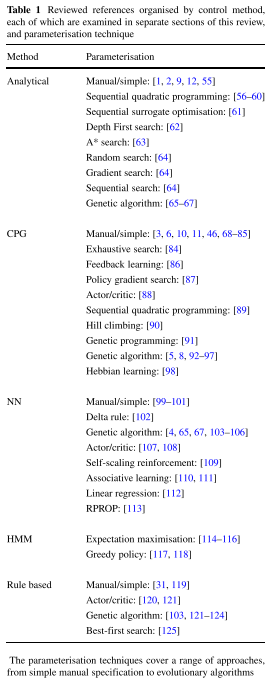
\includegraphics[scale=0.8]{../../images/ParametrizationsTechniques.png}\\
\href{run:/home/jackmaster/Downloads/[2013 Joe Wright and Ivan Jordanov] Art Intelligent approches in locomotion - A reveiw.pdf:pdf}{
\textbf{HMM Algorithm}\\
%The first part of imitation is recognition, where a recursive algorithm calculates the probability of observing a movement pattern, If recognition does not occur, then the next stage of imitation is learning. To synthesize, or produce the movement once stored, it is usually generated stochastically from the HMM. If the pattern is not recognized, then it is added to the database as a new, learned pattern.
\textbf{HMM introduction}\\
%Some research has been conducted into robotic learn-ing by imitation, where the robot goal is to observe a motion pattern and then to reproduce it. the physical workings and capa-bilities of the source and target systems are different, simple copying will not work. Imitation therefore, becomes a process of observation and re-synthesis. Here, observing is estimating the underlying state variables of the source system where only the output is available, and HiddenMarkov Models (HMM) have been used in robotics for this task [114–118].
\textbf{01 Short Content: locomotion control methods and parameter specification techniques}\\
%Among the investigated intelligent approaches for solving locomotion problems are oscillator based Central Pattern Genera- tors, Neural Networks, Hidden Markov models, Rule Based and Fuzzy Logic systems, as well as Analytical concepts. We try to compare those methods based on the quality of the produced solutions in terms of time, stability, correctness and the expense and cost for achieving them. As many of the reviewed techniques require extensive parameter specification, this review also outlines key techniques of learning and optimisation as applied in the field.
}\cite{Wright2014}
\subsection{Estado del arte}
\subsubsection{Control}
El \'enfasis esta sobre modelos y leyes de control para lograr el comportamiento mas simple posible, nombrado, asintoticamente estable, periodico y sobre piso plano. El m\'etodo de Poincare para establecer estas propiedades de orbitas periodicas de sistemas hibridos es desarrollado con el aniomo de ser posible aplicarlo a modelos de dimension superior. Es usado el modelo totalmente dinamico o un modelo simplificado? Si es el ultimo, Como es? Es hibrido, como el impacto tomado en cuenta? Son problemas que permiten modelos subactuados?\\
Un modelo es estudiado donde los pies son remplazados por puntos de contacto. Este puede ser pensado como una marcha en zancos o como la caminata con pies peque\~nos es tal que permite rotaci\'on en los pies, y por lo tanto la subactuacion es inevitable.\\
Una idea importatnte es que un dominio totalmente actuado en el plano sagital y coronal de un bipedo en 3D puede ser desacoplado usando una variante geometrica de reduccion llamada funcional de reducion Routhian.\\
Un gran numero de dise\~nos de control han sido introducidos usando modelos los cuales varian de una representacion simplificada a un modelo de dimension completa. Los modelos simplificados traen consigo beneficios que haces mas tratable el analisis, meroran el conocimiento y las rapida computacion de los controladores. Modelos complejos apuntan a mejorar la habilidad de mejorar la predicion y una forma de garantizar la estabilidad.\\
El ZMP es un punto en el piso en el cual la las fueras de reaccion actuando entre el piso y el pie producen un momento horizontal nulo. Tradicionalmente, la estrategia de control de ZMP logra una caminata al planear el movimiento del centro de masa CoM del robot tal que ZMP permanece strictamente al interior del Convex Hull del pie que se encuentra como soporte en el caso de soporte simple (o en el Convex Hull  de los dos pies cuando se encuentra en doble soporte). Bajo esta condicion de AMP, el piede soporte permanece plano contra el piso y esta inmovil sin rotaci\'on.\cite{Xiang2010}\\
El caso especial del modelo de pendulo lineal invertido, el ZMP puede ser expresado explicitamente en terminos de la dinamica del CoM, tan solo con la linerizacion de una ecuacion diferencial ordinaria. La calve de estas suposiciones es permitir esta simplificacion, incluyendo la representacion de un robot coo una masa puntual con piernas telesc\'opica.\cite{Grizzle2014}\\
Kato comenzo trabajando sobre la serie de robots WABOT en los a\~nos 70. Un robot de escala completa antropomorfica, WABOT-1, fue preortado por Kato, con una marcha estaticamente estable mientras transportaba objetos con sus manos. Una decada despues, la tecnica del ZMP fue por primera vez demostrada en la practica sobre el bipdel WL10-RD.\cite{Grizzle2014}\\
Los metodos ZMP tiene sus limitaciones. Las marchas dise\~nadas con esete metodo generalmetne no tiene en cuenta el impacto, y por lo tanto la trayectoria del pie de balanceo esta dise\~nada de tal forma que no impacte con el piso, llevando una velocidad m\'inima, la condicion ZMP no son suficientes para aproponer una estabilidad asimtotica del movimiento periodico de la marcha.\cite{Grizzle2014}\\
El LIPM con compensacion de la gravedad el cual a\~nade unos puntos adicionales de masa localizados en los pies de balanceo para lograr una mayor presicion de modelo. Los requerimientos de altura del CoMen el LIPM son realajados condiciendo a un modelo de pendulo invertido no lineal. Un volante es a\~nadido en el pendulo invertido; Una gran variedad de modelos de pendulo han sidousados para analizar el equilibrio y la recuperacion despues del impacto.\cite{Grizzle2014}\\
\href{run:/home/jackmaster/Downloads/[2014 Jessy W Grizzle and Christine  Chevallereau and Ryan  W Sinner and Aaron D Ames] Art Survey  paper: Models, feedback control and open problems of 3D bipedal robotic walking.pdf}{
% Control\\
%The emphasis is on models and control laws for achieving the simplest possible behavior, namely, asymptotically stable, periodic, walking on flat ground.\\
%The method of Poincaré forestablishing stability properties of periodic orbits of hybrid systems is developed with an aim at being able to apply it to high-dimensional models.\\
%Does it use the full dynamical model or a simplified model? If the latter, what is it? Are hybrid aspects, such as impacts, explicitly taken into account? Are underactuated models allowed?\\
%A model is studied where the foot is replaced with a point contact. This can be thought of as walking on stilts or as walking with very small feet so that foot rotation, and hence underactuation, is unavoidable.\\
%An important idea is that in the fully actuated domains the sagittal and coronal2 dynamics of a 3D biped can be decoupled using a variant of geometric reduction termed functional Routhian reduction.\\
%Myriad control designs have been introduced using models which vary from the simplified representations shown in Fig. 5 to full-dimensional dynamic models as developed in Section 3. simplified models point to the benefits of more tractable analysis, enhanced insight, and faster control law computation, complex models point to enhanced predictive ability and formal guarantees on stability.\\
%the ZMP is the point on the ground at which the reaction forces acting between the ground and the foot produce no horizontal moment. Traditionally, ZMP control strategies achieve walking by planning the motion of a robot’s CoM such that the ZMP remains strictly within the convex hull of the stance foot in the case of single sup-port (or convex hull of the stance feet, in the case of double sup-port). Under this condition on the ZMP, the stance foot remains flat on the ground and immobile (not rotating)\\
%In the special case of the Linear Inverted Pendulum Model (LIPM), the ZMP can be expressed explicitly in terms of the dynamics of the CoM via a linear ordinary differential equation (ODE). There are key assumptions permitting this simplification, including representing a robot as a point mass with massless telescoping legs.\\
%Kato began working on the WABOT series of humanoid robots around 1970. A full-scale anthropomorphic robot, WABOT-1, was reported in Kato, Ohteru, Kobayashi, Shirai, and Uchiyama (1974) and it demonstrated primitive, statically stable walking while transporting objects with its hands. Over a decade later, the ZMP technique was first demonstrated in practice on the WL10-RD biped in Takanishi, Ishida, Yamazaki, and Kato (1985).\\
%ZMP methods, there are recognized limitations. Gaits designed using this method generally donot take impacts into account, and thus the swing foot trajectory must be designed so that it will impact the ground with minimal velocity, ZMP condition is not sufficient for asymptotic stability of a periodic walking motion\\
%Gravity Compensated LIPM which adds an additional point mass at the location of the swing foot to achieve higher modeling accuracy. the requirement of constant CoM height on the LIPM was relaxed leading to a nonlinear inverted pendulum model. a flywheel is added to the inverted pendulum; The various pendulum models have been widely used in analysis of push recovery and balance\\
}\cite{Grizzle2014}
El puntos de captura es un putno en el piso sobre el cual el bipedo puede dar el paso y detenerse completamente si caer; El punto de captura (Tedrake) ha ganado reconocimiento y se a convertido en un putno de estabilizacion del bipedo. Los modelos de resorte cargdos de pendulo invertido (SLIP), los cuales han sido mostrados para aploximar el centro de masa del cuerpo durante el movimiento en estado de marchas estable de corrida en una amplia diversidad de animales terrestres. El control de estos robots puede ser descompuesto en tres subtareas dedicadas a: a) propulsion hacia adelante del robot a una velocidad deseada, b) regulacion vertical de la altura del cuerpo en el salto, y c) mantener el cuerpo en una postura deseada. Para controlar la velocidad de avance, el controlador coloca los dedos del pie en una posicion deseada con respecto al centro de masa durante el vuelo. Para regulara la altura del salto, las longitudes de las piernas sobre laparte inferior del la fase de soporte es ajustada al dar una cantidad fija de soporte. Para controlar el avancedel cuerpo, el controlador emplea un torque en la cadera en durante la fase de soporte. El dise\~no de los robots PWD con dinamicas aproximadas a realizar un modelo simplificado. La estabilidad d\'inamica es lograda m\'as por el dise\~no mecanico que por el control por realimentaci\'on. Los investigadores que siguen este camino generalmente consideran la dinaica del impacto. Mochon y McMohon concluyen que la fase de balnceo de la marcha humana es similar a la de pendulo doble, argumentando que la naturaleza pasiva de la marcha humana y la importancia en su dise\~no.\cite{Grizzle2014}\\
Los metodos basados en energ\'ia  para dise\~nar estrategias de control basado en pasividad con los controladores simetricos, metodos modernos han logrado mejorar el control por la formulacion del problema de control como una programacio cuadratica (QP), permitiendo a las marchas remplazar sobre la ejecucion y mejorando las propiedades de estabilidad. Los metodos de suma de cuadrados, tambien furmulan la genracio de trayectorias como una optimizacio convexa. Se garantiza la estabilidad. Los procedimientos investigan la nocion de controlabilidad, formando embudos o canales sequenciales (verificando la desigualdad de suma de los cuadrados de Lyapunov), para el cual cad uno conduce a un conjunto predefinido de objetivos. Crear una trayectoria con propuedades de estabilidad garantizados: sobre cualquier punto dado en timepo, el sistema esta dentro de un canal o region de atraccion\cite{Grizzle2014}
Subactuados: control por realimentacion de un un bipedo con un punto de contacto por modelo corresponde a caso limite cuando lospies del robot, como tama\~no se reducen a cero. Entonces el pie plano con actuacion en el pie puede ser acompa\~nado con ()torques qeu respetarn las restricion de no retacion alrededor de un aborde del pie de soporte. (Adios al ZMP?). una restricion es definida como virtual si esta es lograda atravez del control realimentado en lugar de atravez de las conexiones fisicas, como en el caso de los engranes o las condicones de contacto con los alrededores.\\
Las restriciones virtuales y la dinamica cero hibrida originada en el estudio de la subactuacion, locomocion bipeda plana, intenta describir la marcha caminata, como las diferencias entre la marcha humana (con flexion de rodilla hacia adelante) y la caminata de pajaros (con flexion de rodillas hacia atras), o el torso siendo vertical contra inclinarlo hacia adelante, lleva a una descripcion de posturas o formas del robot por un paso. La misma idea es palicada a robots en 3D, con la adicion de coordenadas parametrizadas la evolucion del robot dentro su plano frontal y su rotacion Yaw.\cite{Grizzle2014}\\
Que tipo de estabilidad es obtenida?\\
Nosotros necesitamos la nocion de dinamica cero y la invarianza hibrida para definir restricciones iguales y desiguales. Y finalmente la dinamica cero hibrida es creada. Un pregunta de analisis: Para una orbita periodica dada cero y una selecion de restricion virtual (en general, diferentes para cada dominio), cuando conducira y asimtoticamente llevada a cero en una robita estable (resp. asintoticamente estable o expnencialmetne stable?)\\
Como dise\~nar un controlador realimentado para satisfacer multiples requerimientos?\cite{Grizzle2014}\\
\href{run:/home/jackmaster/Downloads/[2014 Jessy W Grizzle and Christine  Chevallereau and Ryan  W Sinner and Aaron D Ames] Art Survey  paper: Models, feedback control and open problems of 3D bipedal robotic walking.pdf}{
%the capture point — a point on the ground on which a biped can step and come to a complete (upright) stop without falling over; The capture point (Pratt and Tedrake, 2006) has gained recognition as a convenient method for stabilizing a biped.\\
%the Spring-Loaded Inverted Pendulum (SLIP) model, which has been shown to approximate the body center-of-mass (CoM) motion during steady-state running gaits of a wide diversity of terrestrial animals. The control of these robots can be decomposed into three subtasks dedicated to (a) forward propulsion of the robot at the desired speed, (b) regulation of the vertical hopping height of the body, and (c) keeping the body at a desired posture. To control the forward speed, the controller places the toe at a desired position with respect to the center of mass during flight. To regulate the hopping height, the length of the leg at the bottom of the stance phase is adjusted by giving a fixed amount of thrust. to control the pitch attitude of the body, the controller employs hip torque during stance.\\
%PWD design robots with dynamics that approximately realize a simplified model. dynamic stability is achieved as much as possible through mechanical design instead of feedback control. researchers who follow this path often consider impact dynamics,\\
%Mochon and McMahon (1980) concluded that the swing phase of human walking is similar to a double pendulum, pointing to the passive nature of human walking and the importance of mechanism design.\\ 
%energy-based methods to design passivity-based control strategies such as controlled symmetries,\\
%Modern methods have achieved improved control by formulating the control problem as a quadratic program (QP), allowing gait replanning on the fly and improving stability properties. sums of squares methods, also formulate trajectory generation as a convex optimization. guarantees on stability The procedure investigates the notion of controllability, composing sequential funnels (verified with sum of squares Lyapunov inequalities), which each lead to a predefined goal set. create a trajectory with guaranteed stability properties: at any given point in time, the system is within one of the known funnels (regions of attraction).\\
%Underactuated: feedback control of a biped with the point-foot contact model corresponding to the limiting case of a robot with feet, as the size of the feet decreases to zero. then flat-footed walking with actuated feet (of any size) can be accomplished with (arbitrarily small) torques that will respect the constraint of no rotation about an edge of the stance foot,(Good bye to ZMP?)\\
%Virtual constraints and hybrid zero dynamics originated in the study of underactuated, planar bipedal locomotion in\\
%attempt to describe a walking gait, as the difference between human-like walking (knees bent forward) and bird-like walking (knees bent backward), or the torso being upright versus leaning forward, leads to a description of the posture or shape of the robot throughout a step. The same idea applies to a 3D robot, with the addition of coordinates parameterizing the robot’s evolution in the frontal plane and its yaw rotation.\\
%Which kind of stability is gotten?\\
%We need the notion of zero dynamics and hybrid invariance to define equal and inequal constraints. And finally Hybrid zero dynamics is created. An analysis question: For a given periodic orbit O and selection of virtual constraints (in general, different for each domain), when will driving y in (55) asymptotically to zero render the orbit stable (resp., asymptotically stable, or exponentially stable)?\\
%How to design a feedback controller to satisfy multiple requirments?\\
}\cite{Grizzle2014}
La optimizacion con el uso de polinomios de Bezier, para dise\~no de marcha necesita de una parametrizacion finita de las restriciones virtuales: esto es un problmea de optimizacion con restricion no lineal. Una pregunta a sintetizar: Como dise\~nar una restriccion virtual, y controles por realimentaci\'on tal que imponga la propiedad asintotica, el cual coloca lleva a una orbita periodica estable y asintotica conociendo los requerimientos motivados fisicamente como: la eficiencia energetica el robot camina a una velocidad deseada; \\
la fuerzas de reaccion sobre las piernas requieren una restricion unilateral? cuando un robot ha tenido pies que no son triviales, el puen puntual en la estrategia de ocntorl presenta dificultades si las siguientes inconvenientes no son tomados en cuenta: El motodo propuesto puede ser visto como una modificacion online de las trayectorias de referencia en orden de asegurar satisfaccion de las restriciones de contacto.\cite{Grizzle2014}\\
Motivado por la literatura de la biomecanica, la marcha humana puede ser usada para inspirar la construccion de modelos sistema hibridos, sobre restricciones virtuale, inspiradas por los datos de locomocion humana, que llevana a caminatas estables.\\
A la fecha, el dise\~no de dinamica cero sobre actuadores SEA ha sido orientada en dos caminos: el modelo de resortes, que fue tomado asumiendo que si las variables de control h0 de las articulaciones al lado de los resotes, el grado de estos componentes llega a ser 4 en lugar de 2, y la dinamica cero del robot con una actuacion elastica en serie es difeomorfa (hace referncia a un isomorfismo de manifolds o variedades suaves o difernciables) para ese robot con actuacion elastica en serie SEA. Grado 2 de salidas en mucha mas sencilla de calcluar e implementar que un controlador basado en 4 grados de salida relativa.\cite{Grizzle2014}\\
Lyapunov y restricciones virtuales\\
Muestra que no es necesario linearizar el mapeo de etrada-salida; tan solo la habilidad de sintonizar la razon de convergencia exponencia es lo importante. El control rapidamente estavilizado de Lyapunov es experimentado en la plataforma MABEL\\
La reduccion Routhiana
El funcional de reduccion Routhiana ha sido util para lograr la caminata en 3D en un numero de bipedos en simulacion, y tambien ha sido demostrado en la practca. La formacion de la enervia del bipedo a traves del control, el funcional de reduccion Routhiana puede efectivamente desacoplar la dinamica sagital y coronal de un bipedo 3D permitiendo un dise\~no de control exclusivo paa la dinamica del plano sagital\cite{Grizzle2014}\\
\href{run:/home/jackmaster/Downloads/[2014 Jessy W Grizzle and Christine  Chevallereau and Ryan  W Sinner and Aaron D Ames] Art Survey  paper: Models, feedback control and open problems of 3D bipedal robotic walking.pdf}{
%Optimization via Bezier polinomials Gait Design needs a finite parametrization of the virtual constraints: that is a nonlinear constrained optimization problem. A synthesis question: how to design virtual constraints, and feedback controllers that asymptotically impose them, which together yield an asymptotically stable periodic orbit meeting physically motivated requirements such as: energy efficiency; the robot walks at a desired speed; and the reaction forces at the leg
%end respect required unilateral constraints?\\
%When a robot has nontrivial feet, the point-foot control strategy presented in Section 5 can be applied without difficulties if the following additional issues are taken into account\\
%The proposed method can be viewed as an on-line modification of the reference trajectory in order to ensure the satisfaction of the contact constraint.\\
%Motivated by the biomechanics literature,30 human-walking can be used to inspire the construction of hybrid system models, along with virtual constraints – inspired by human locomotion data – that yield provably stable walking gaits.\\
%To date, the design of the zero dynamics for series elastic ac-tuators has been addressed in two distinct ways. the spring model of Spong (1987) was adopted. It (q) are taken on the was shown that if the controlled variables h0 joint side of the spring, the relative degree of those components of the output becomes 4 instead of 2, and the zero dynamics of the robot with series elastic actuation is diffeomorphic to that of the robot without series elastic actuation. degree 2 outputs is simpler to compute and implement than the controller based on relative degree 4 outputs.\\
%Lyapunov and virtual constraints\\
%shows that it is not at all necessary to linearize the input–output map; it is only the ability to tune the rate of exponential convergence that is important. Rapidly Exponentially Stabilizing Control Lyapunov validated experimentally on MABEL\\
%Routhian reduction\\
%functional Routhian reduction has been helpful in achieving 3D walking in a number of bipeds in simulation, and has also been demonstrated in practice By shaping the energy of a biped through control, functional Routhian reduction can effectively decouple the sagittal and coronal dynamics of a 3D biped and allow for control design to be conducted with the dynamics restricted to the sagittal plane.
}\cite{Grizzle2014}
\subsubsection{Control de caos}
Los bipedos pasivos son sistemas dinamicos los cuales son sensitivos a las condiciones iniciales debido a que estos exhiben un comportamiento ca\'otico. Varias dinamicas caoticas, bifurcaciones, intermitencias y crisis, ocurren como consecuencia de la variacion en diferentes parametros de las equaciones din\'amicas de muchos modelos simples de caminadores pasivos. Las investigaciones en caos de los bipedos PWD ha emergido interdisciplinariamente y son utilies en la diagnosticacion de marchas patologicas.\cite{Iqbal2014}\\
\textcolor{red}{Tendencias futuras} Las futuras aplicaciones requiere que estos robot caminen y corran en entornos no estructurado y no familiares. Como los terrenos irregulares, el sistema dinamico puede llegar a comportamientos caoticos.\cite{Iqbal2014}
\subsubsection{Redes neuronales}
\subsubsection{Central pattern generators}
El control de la locomocion ha sido resuelto basado principalmente sobre mecanismos programados. Para usar este metodo, las trajectorias de camiata para cada pierna y marcha deben ser dise\~nados, y la adaptabilidad de entornos desconocidos no puede ser garantizada. Por que los humanos tiene como tal un buen movimiento ritmico? Los biologos creen que generador de patrones centrales (CPG) es la respuesta a esta pregunta. CGP es una clase de red neuronal que puede endogenicamente producir un patron ritmico en sus salidas. Este esta distribuido atraves de la parte inferior toraxica y la region lumbar de la columna vertebral y es responsable de distintos patrones de marcha.\cite{Wu2009}\\
los CPG tienen muchas caracteristicas:\cite{Wu2009}\\
1) control periodico de se\~nales aun sin ningun tipo de sensor a la entrada y ordenes  superiores. Como sea, las entradas sensoriales y las ordenes superiores puede modular la actividad del CPG. Los robots prefierne caminar en un camino plano con un control de lazo abierto o adaptarse al caminar sobre un terreno irregular con un lazo cerrado de control.\\
2) le metodo es un control distribuido. Una unidad CPG controla una articulacion de un robot, y una red de CPG coordina todas las articulaciones para completar el movimiento. Mediante modulacion de los parametros de la red CPG, puede lograrse diferentes marchas.\\
3) Adaptacion al entorno, el proceso de planeacion del movimiento es seprado con el control en lazo cerrado en el metodo tradicional de programaci\'on. El sistema neural produce se\~nales para controlar el cuerpo para moverse en un entornot. La reacion del entorno a las modificaciones del cuerpo, los parametros del sistema neuronal para cambiar las se\~nales de control.\\
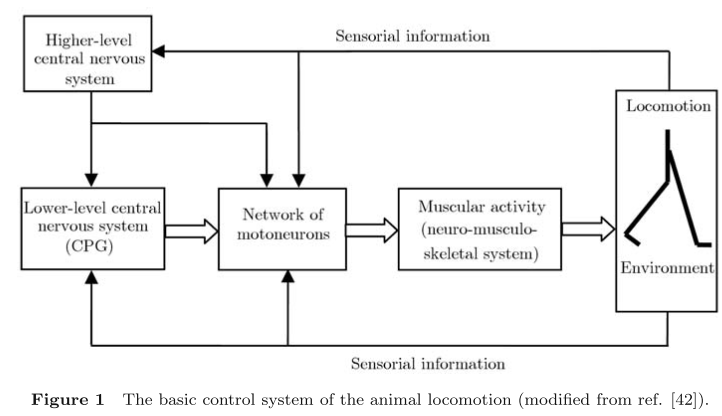
\includegraphics[scale=0.4]{../../images/CPGBasicControlSystem.png}\cite{Wu2009}\\
Desarrollo biologico del CPG\\
Intestigacion neurobiologica:
\begin{itemize}
\item Teoria del reflejo (\emph{Reflex theory}): Basado en la realimentaci\'on del est\'imulo perif\'erico, los efectores deben ser activados por los sensores de realimentacion y las partes moviles del cuerpo (Se ha probado que es irrasonable).
\item Teor\'ia del CPG: Aunque el CPG se ha probado que funciona, aun sigue siendo controversial.
\end{itemize}
Las propiedades del CPG\\
\begin{itemize}
\item CPG existen en los cuerpos animales.
\item CPG esta constituido por una varias unidades acopladas entre si.
\item CPG preduce se\~nales ritmicas por si solo, sin embargo las ordenes superiores y la realimentacion de su entorno podrian modular las salidas del CPG
\end{itemize}
Controlador neural de la caminata en los vertebrados. Entonces las se\~nales finales de control de la caminata, son el resultado de la interaccion mutua entre el sistema nervioso central y el sistema de reflejos. El nivel mas superior del sistema nervioso central envia ordenes. Entonces, el CPG produce unas se\~nales ritmicas y estas se\~nales son pasadas al sistmea musculo-esqueletico por las neuronas motoras para generar el movimiento. Por ultimo, el cuerpo recive una informacio de vuelta y los reflejos producen unos comandos de movimiento adicionales. Un nuevo ciclo comienza.\\
\href{run:/home/jackmaster/Downloads/[2009 Wu QiDi and Liu ChengJu and Zhang JiaQi and Chen QiJun] Art Survey of locomotion control of legged robots inspired biological concept.pdf}{
%locomotion control has been solved mainly based on programming mechanism. To use this method, walking trajectories for each leg and the gaits have to be designed, and the adaptability to an unknown environment cannot be guaranteed\\
%Why does human has such a good rhythmic movement? Biologists believe that central pattern generator (CPG) is the answer to this question. CPG is a kind of neural network that can endoge-nously produce rhythmic patterned outputs[3−5].It is distributed throughout the lower thoracic and lumbar regions of the spinal cord and responsible for different walking patterns[6,7].\\
%CPG has many features: \\
%(1) periodic control signals even without any sensory inputs and higher orders. However, the sensory inputs and higher orders can modulate the activity of CPG. robots can either walk on flat terrain with an open loop control or adaptively walk on irregular terrain with a closed loop control.\\
%(2) distributed control method. one CPG unit controls one joint of a robot, and a CPG network coordinates all joints to complete a movement. By modulating the parameters of a CPG network, can be used to acquire different gaits.\\
%(3) adapt to the environment. motion planning process is separated with the control loop in the traditional programming method. The neural system produces signals to control the body to move in an environment. The reaction from the environment to the body modifies the parameters of the neural system to change control signals.\\
%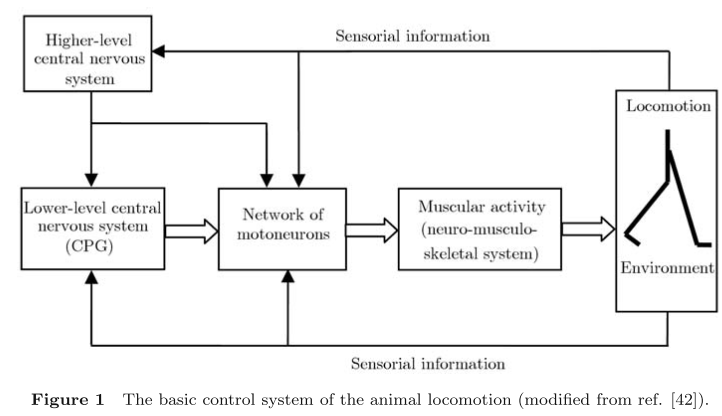
\includegraphics[scale=0.4]{../../images/CPGBasicControlSystem.png}\\
%BIOLOGICAL DEVELOPMENT OF CPG\\
%Neurobiology research
%\begin{itemize}
%\item Reflex Theory: Based on feedback of peripherial stimulus-> The effectors must be activated by feedback of sensor and moving parts  of the body (Proved to be unreasonable).  
%\item CPG Theory: Whether CPG  works on is still controversial.
%\end{itemize}
%The properties of CPG
%\begin{itemize}
%\item CPG is existed on animal bodies 
%\item CPG is make up by one or several units coupled together 
%\item CPG produced rythmic signals by itself, but higher order and feedback from enviroment would modulate output signals from CPG
%\end{itemize}
%Walking control network of vertebrates\\
%So, the final walking control signals are the result of the mutual interaction of central nervous system and reflexes system.  Higher-level central nervous system sends orders. Then, CPG produces rhythmic signals and these signals are passed to musculo-skeletal system by motoneurons to generate a movement. Last, body receives feedback information and reflexes to produce further  movement commands. A new loop begins.\\
}\cite{Wu2009}\\
Los osciladores neurales denomiados generadores de patron central CPG, proveen el ritmo basico para la actividad muscular durante la locomocion. Un modelo CPG, el cual automaticamente se sintoniza dentro de sus frecuencias de resonancia a los caminadores bipedos de dinamica pasiva. El comportamiento en la  sintonizacion de la resonancia del modelo CPG permite a la velocidad de la marcha ser controlada de por un parametro individual, mientras mantiene la eficiencia energetica de la caminata dinamica pasiva.\cite{Verdaasdonk2009}\\
Los osciladores neurales en la columna vertebral, denomiados CPGs, juegan un papel fundamental para sumismtriar la energia de forma eficiente durante la caminata humana. Los CPG exitan los musculos de una forma periodica, dando cabida a una locomocion estable. El modelo simple de las CPG permite la entrega ritmica eficiente sobre cada movimiento de pierna por separdo. No existe una evidencia directa del CPG en la que en el cuerpo humano halla sido encontrado.\cite{Verdaasdonk2009}\\
\textcolor{red}{Un sistema CPG con sistema musculo-esqueletico central crea un ciclo l\'imite estable el cual es bastante robusto contra las perturbaciones, la eficiencia energ\'etica es obtenida al sintonizar el sistema musculo-esqueletico en las frecuencias de resonancia.} Los modelos dem caminata pasiva dinamica para cada pierna estan localmente acoplados con su propio CPG sobre la articulacion de la cadera aferentes y eferentes, asosciado los sensores de realimentacion y el sistema motor, respectivamente. La eficiencia energetica depende 1) la habilidad del oscilador neural de sintonizar las frecuencias de resonanciaa y 2) la energ\'ia perdida por la amortigaci\'on, durante la fase de despejo del piso (para evitar el tropiezo) es provocado artificialmente. La frecuencia de zancada, su frecuencia natural es cambiada al colocar una resistencia rotacional en la cadera Kh.\cite{Verdaasdonk2009}\\
Un modelo con resistencia Kh=0 recrea el modelo minimalista de la caminata dinamica pasiva, tal que el modelo mas simple (Garcia) y el modelo de marcha del comp\'as (1997), nuestro modelo del contacto del pie-suelo es modelado por una amortiguacion viscosa en ambas direcciones $x$ e $y$ y la resistencia solo afecta la direccion $y$, es posible la investigacion de la caminata en diferentes tipos de pisos (por ejemplo las superficies lisas o deslizantes). Ahora el modelo en tiempo continuo, permite caminar \emph{por siempre} en lugar de un paso a la vez. Se usa un sistema de cuatro coordenadas generalizadas, que involucra la posicion global de la cadera en el espacio y los angulos relativos de cada pie respecto a la verticual.\cite{Verdaasdonk2009}\\
Realimentacio posicional, integral y derivativa de los angulos de laspiernas a los centros del CPG flexores y extensores. El efecto posicional prevee la sintonizacion de la resonancia arriba de la frecuencia endogeica del CPG, fCPG. La accion integral otorga la sintonicacion de la resonancia resonancia debajo de la frecuencia fCPG. Para compensar la velocidad en el retardo de tiempo acoplado a cada piernta del CPG. Sin freno actuvo de las piernas  es necesario y en consecuencia solo trabajo positivo es realizado por los musculos de la cadera. La resistencia Kh, incrementar la velocidad de la marcha de un caminador controlado por CPG es obtenido al incrementar el gasto energetico de los musculos.\cite{Verdaasdonk2009}\\
CPG logra el control de caminadores pasivos con un gato similar en terreno plano comparado con la caminata de dinamica pasiva, mientras alcanza velocidades que superan en gran medida las regiones de estabilidad de los PWD. En el primer metodo (ajuste de la resonancia) parace una mejor alternativa, porque para los caminadores de dinamica pasiva con rodillas mas sofisticados, lospies y la forma que almacenan la energia cinetica ahora es perdida al momento del choque del talon (tendoones) la energia cinetaica pierde  puede ser minimizada, mientras no actuen el caminador  en su dinamica natural (en eigen modo) siempre llevara a la perdida de energia. La manera mas eficiente de actuar un oscilador mecanico, en este caso un PWD, es sobre su frecuencia de resonancia (Afinacion resonante). Sin la realimentacion de la velocidad es imposible sintonizar la resonancia para zancadas de frecuencia altas. Desde que los CPG actuan los PWD sonre su frecuencia de resonancia, los cambios de velocidad se pueden llevar a cabo por el cambio de la longitud de la zancada. En el modelo de \cite{Verdaasdonk2009}, se puede vislumbrar como los humanos logran alcanzar marchas de eficiencia energetica y tambien se puede usar como un controlador de la marcha en aplicaciones como dispositivos energizados para ortesis.\\
\href{run:/home/jackmaster/Downloads/Doc Thesis/Walkers/[2009 B W Verdaasdonk and H F J M Koopman and F C T van der Helm] Art Energy efficient walking with central pattern generators: from passive dynamic walking to biologically inspired control.pdf}{
%neural oscillators termed central pattern generators (CPGs) provide the basic rhythm formuscular activity in locomotion. a CPG model, which automatically tunes into the resonance frequency of the passive dynamics of a bipedal walker\\
%The resonance tuning behavior of the CPG model allows the gait velocity to be controlled by a single parameter, while retaining the energy efficiency of passive dynamic walking.\\
%Neural oscillators in the spinal cord, termed central pattern generators (CPGs), are likely to play a key role in providing energy efficient human gait\\
%CPGs excite the muscles in a periodic fashion, giving rise to stable locomotion.\\
%simple model of a CPG is able to provide energy efficient rhythmic single limb movement\\
%no direct evidence of CPGs in the human body has been found yet,\\
%CPGs with the musculo-skeletal system and its environment creates a stable limit cycle which is quite robust against perturbations\\
%The energy efficiency is obtained by tuning into the resonance frequency of the musculo-skeletal system.\\
%passive dynamic walking model each leg is locally coupled to its own CPG at the hip joint afferent and efferent, associated with sensory feedback and motor control, respectively. energy efficiency depends (1) ability of the neural oscillator to tune into the resonance frequency (2) energy losses by damping, ground-clearance during swing phase is provided artificially. stride frequency its ‘resonance frequency’—is changed by adding rotational hip stiffness Kh.\\
%model without hip stiffness (i.e. Kh =0) resembles minimalistic models of passive dynamicwalking, such as the ‘simplest walking model’ (Garcia et al. 1998) and the ‘com-pass gaitmodel’ (Goswamiet al. 1997). our model foot-ground contact modeled by viscous damping in both x- and y-direction and stiffness only in y-direction investigation of walking on different types of ground (e.g. a slippery surface) possible, Our model is a continuous-time model, able to walk ‘forever’ instead of one step at a time.We four generalized co-ordi-nates q =[xh yh θr θl]T, in which xh and yh are the co-ordi- nates of the hip massmh parallel and perpendicular to ground nates q =[xh yh θr θl]T, in which xh and yh are the co-ordi- nates of the hip massmh parallel and perpendicular to ground level,\\
%Posi-tional, Integral and Derivative feedback of the limb angle to the flexor and extensor centers of the CPG. positional provide res-onance tuning above the CPG’s endogenous frequency fCPG. Integral provide resonance tuning at and below fCPG. velocity compensate for the time delay in the loop coupling limb to the CPG. Resonance.\\
%no active braking of the legs is necessary and thus only positive work is performed by the hip muscles.\\
%hip stiffness Kh, increasing gait velocity v of the CPG-controlled walker is achieved by increasing the energy expenditure of the muscles.\\
%CPG achieves con-trol of the passivewalker with similar energy expenditure on flat ground compared to passive dynamic walking, while it can achieve speeds that greatly exceed the region of stability of passive dynamic walking.\\
%The former method (i.e. resonance tuning) seems a better alternative, because for a more sophisticated passive dynamic walker with knees, feet and a way to store the kinetic energy now lost at heel strike (e.g. tendons) the kinetic energy losses can be minimized, while not actuating a passive dynamic walker in its natural dynamics (i.e. eigenmode) will always mean energy losses.\\
%The most efficientway to actuate a ‘mechanical oscillator’—in this case a passive dynamic walker—is at its resonance frequency (i.e. resonance tuning).\\
%without velocity feedback resonance tuning is not possible at high stride fre-quencies.\\
%Since the CPG actu-ates the passive dynamic walker at its resonance frequency, the velocity change will be achieved by a change in stride length.\\
%Our CPG model on the one hand might elucidate how humans achieve energy efficient walking, and on the other hand can be used as (part of a) gait controller in applications such as walking robots or powered walking orthoses.
}\cite{Verdaasdonk2009}
\subsubsection{Hidden Markov}
\textcolor{red}{Posible intro para HMM} Algunas investigaciones has sido conducidas al interiorn del aprendizaje por imitaci\'on, donde el objtivo del robot es observar un patron de movimiento y luego reproducirlo. Las plataformas construidas y sus capacidades se diferencias de los seres vivos a quienes se intenta imitar, y se ha observado que esta simple copia no funciona. La imitaci\'on por lo tanto, se convierte en un proceso de observacion y re-s\'intesis. Aqu\'i observar es estimar el estado intriseco de las variables de estado del individuio a imitar donde solo es posible ver las se\~nales de salida y es aca donde los modelos ocultos de Markov han sido usados.\cite{Wright2014}\\
El argoritmo de imitaci\'on usando Modelos Ocultos de Markov, procede globalmente as\'i 1) Reconocimiento del patr\'on de moviento: Un algoritmo recursivo calcula la probabilidad de observar un patron de movimiento, si no es reconocido 2) el siguiente paso es el aprendizaje:  se crea un nuevo modelo oculto que sintetiza los patrones de movimiento. 3) Finalmente el movimiento es almacenado como un nuevo patron aprendidio y luego es reproducido.\cite{Wright2014}\\
\textcolor{red}{Capa cognitiva alta} Ventajas: imitar, alta precision para replicar trayectorias, aprender multiples habilidades. Desventajas: No es intrinsecamente adaptable, no puede proponer nuevos movimientos, no funciona por si solo requiere otras t\'ecnicas.
\subsubsection{Sistemas basados en reglas}
Al conocer el estado actual y la siguiente acci\'on del caminador puede ser determinada a traves de una tabla de consulta o una sistema basado en reglas. El uso de un agente experto en conocimiento o tecnicas de optimizacion y aprendizaje son usadas para especificar dichas reglas de transisi\'on. Tablas generadas generalmente en la literatura por Algoritmos Gen\'eticos.\cite{Wright2014}\\
Algunos ejemplos encontrados: 1) un controlador difuso b\'ipedo basado en ZMP logra unas marchas m\'as deseables al tener menos balanceos en el tronco. El control es aplicado para variar la posicion del ZMP en el rect\'angulo de soporte. 2) Un control para una plataforma bipeda para subir escaleras, un control difuso parametrizado con GAs doble es usado, el primero para analizar el estado actual y el segundo para predecir la siguiente accion a tomar. El desempe\~no de este controlador es comparado con otros usados con redes neuronales y logica difusa. Segun los autores, el controlador difuso mostro mejor desempe\~no que el control ZMP con modelo de p\'endulo invertido. Sin embargo el mejor de todos se reporta usando redes neuronales.\cite{Wright2014}\\
Ventajas: Facilidad para implementar, las reglas son interpretables y puede ser usado un agente experto, faciles de optimizar, pueden enfrentar varios ambientes o condiciones de terreno. Desventajas: Sirve para movimientos bastos o bruscos, los m\'etodos estan sobre restringidos y presentan un menor potencial de optimizaci\'on.\cite{Wright2014}\\
\subsection{Futuras tendencias}
\subsubsection{Control}
Cualquier investigador conociendo este problema b\'asico y puede asegurar que existe mas interes en las marchas aperiodicas, terrnos no planos, maniobras, marcha en modo de correr, eficiencia energetica, autonomia y muchas mas. Existe una buena rason para creer que una marcha constituida por mas de una ciclo de marcha completo, golpe del tal\'on, pie plano, rodadura de la punta del pie, pueden ser realizados de una forma estable. El punto de contacto es potencialmente m\'as dificil de controlar que los que tienen golpe en el talon y rodadura en la punta del pie.\cite{Grizzle2014}\\
El trabajo de chevallereau  muestra que aun en el caso de la caminata con pie plano y tobillo actuada, si el sentro de presion de la fuersa de reaccion del piso sobre el piede apoyo esta contrlada activamente con la intension de evitar la rotacion del pie, el corespondiente porblema de control es subactuado. Por esta misma razon, la caminata con un pie puntal subactuado presenta una prueva interesante en el caso de cualquier metodologia de dise\~no para el control.\cite{Grizzle2014}\\
Los resultados en 3D aun siguen estando en su infaciay mucho trabajo falta por hacer. El dise\~no de las restricciones virtuales sobre la base del costo mecanico de transporte es realizado por (). Cuando las restriciones virtuales son dise\~nadas para minimizar la funcionde costo, estos controladores tienden a urealizar un menor esfuerzo.\cite{Grizzle2014}\\
Para un robot evolucionando en 3D, con dos o mas grados de subactuacion, crear un manifold h\'ibrido e invariante es mas desafiante. Los hasta ahora conocidos metodos para lograr la invarianza bajo las pruebas de mapeo son usar la extencion h\'ibrida del pulso muerto(hybrid deadbeat). El mapeo restringido de Poincare resultante de dimension tres o superior, y condiciones para la estabilidad orbital asimtoptica dependen dela eleccion particular de la restriccion virtual usado para parametrizar la orbita con se illustra aqui.\cite{Grizzle2014}\\
Una extension de un enfoque de control subactuado a totalmente actuado  con pies que actual regulando la evolucio de el ZMP presentado por().\cite{Grizzle2014}
\href{run:/home/jackmaster/Downloads/[2014 Jessy W Grizzle and Christine  Chevallereau and Ryan  W Sinner and Aaron D Ames] Art Survey  paper: Models, feedback control and open problems of 3D bipedal robotic walking.pdf}{
% Control Futuras tendencias\\
%Any researcher mastering this basic problem can be assured that there is plenty more to do in terms of investigating, aperiodic gaits, non-flat ground, maneuvering, running, energy efficiency, autonomy, and much more. there is good reason to believe that a gait consisting of a more complete walking cycle, heel strike, flat foot, toe roll, can be realized in a stable manner.\\
%point of contact is potentially more difficult to control than the heel-strike or toe-roll work in Chevallereau et al. (2008) shows that even in the case of flat-footed walking with an actuated ankle, if the center of pressure of the ground reaction forces on the stance foot is actively controlled in order to avoid foot rotation, the corresponding control problem is underactuated. For these reasons, walking with unactuated point feet presents an interesting test case for any control design methodology.\\
%The 3D results are still in their infancy and much work remains to be done.\\
%The design of virtual constraints on the basis of the dimensionless cost of mechanical transport is performed in Ramezani, Hurst, Akbari Hamed, and Grizzle (2014, Eq. (17)) and Sreenath et al. (2011, Eq. (40)).\\
%when the virtual constraints are designed to minimize a cost function such as (70), they tend to use low control effort which means that the ‘‘nat-ural dynamics’’ are used as much as possible instead of being can-celled.\\
%For a robot evolving in 3D, with two or more degrees of underactuation, creating hybrid invariant manifolds is much more challenging. The only known method to achieve invariance under the rest maps is to use a deadbeat hybrid extension. The resulting restricted Poincaré map is of dimension three or higher, and conditions for asymptotic orbital stability depend on the particular choice of the virtual constraints used to parameterize the orbit, as was illustrated here.\\
%An extension of the underactuated control approach to fully actuated robots with feet which acts by directly regulating the evolution of the ZMP was presented by
}\cite{Grizzle2014}
\subsubsection{Dise\~no de CPGs}
Direcciones de investigaciones\cite{Wu2009}
\begin{itemize}
\item Modulacion de parametros: controles especiales de control
\item Restriciones de marcha: Necesidad de coordinar ordenes superiores, CPG y reflejos
\item Estabilidad por el entorno: Dise\~no de lazos cerrados
\end{itemize}
\href{run:/home/jackmaster/Downloads/[2009 Wu QiDi and Liu ChengJu and Zhang JiaQi and Chen QiJun] Art Survey of locomotion control of legged robots inspired biological concept.pdf}{
%Research directions:
%\begin{itemize}
%\item Parameter modulation: special signal control
%\item Gait transitions: Needs to be coorditated higher orders, CPG and reflexes.
%\item Environment stabillity: Design of feedback loops
%\end{itemize}
%Fin
}\cite{Wu2009}
\subsubsection{Basin de atraccion con LQG-tree}
\subsection{Problemas conocidos}
\subsubsection{Adaptabilidad al terreno}
Control de locomocion ha sido resuelto principalmente basado en la programacio del mecanismo. Para usar este metodo, las trayectoias de caminata de cada pierna y marcha tiene que ser dise\~nada y adla adaptabilidad a un entorno desconocido no puede ser garantizado\cite{Wu2009}\\
Los problemas existentes son:\cite{Wu2009}
\begin{itemize}
\item Control de locomocion de robots inpirados biologicamente tiene que ser basados en investigaciones neurobiologicas. Estas herramientas de desarrollo investigativas para probar los problemas correspondientes en otros temas. Trabajar en las se\~nales de control de alto nivel y no solo en CPG.
\item Diferncias entre los actuadores y los musculoas forman una limitacion mec\'anica.
\item Generar se\~nales de coontrol especiales que realmente trabajen en patrones de caminata.
\item Analizar el sistema completa, es dificil y complejo para la eleccion de los parametros o la estabilidad.
\end{itemize}
\href{run:/home/jackmaster/Downloads/[2009 Wu QiDi and Liu ChengJu and Zhang JiaQi and Chen QiJun] Art Survey of locomotion control of legged robots inspired biological concept.pdf}{
%locomotion control has been solved mainly based on programming mechanism. To use this method, walking trajectories for each leg and the gaits have to be designed, and the adaptability to an unknown environment cannot be guaranteed\\
%The existing problems:
%\begin{itemize}
%\item The biologically inspired robots locomotion control has to be based on neurobiological research. This research develop tools to test corresponding problems in other subjects. Working in the high level control signals not only in CPGs.
%\item Difference between actuators and muscles form a limitation on mechanical hardware.
%\item Producing special control signals that really works on walking patterns
%\item Analyze the whole system, is complex and difficult to choose parameter or stabillity
%\end{itemize}
}\cite{Wu2009}
\subsubsection{Control}
La naturaleza de la interfase del pie-piso tambien determina los grados de actuacion (o subactuacion) de los correspondientes modelos dinamicos. Yb oue un rotacion necesariamente lleva a la subactuacion, mientra que si el pie esta plano sobre el piso y todas las articulaciones del robot son actuadas independientemente, el modelo es tipicamente totalmente actuado.\cite{Grizzle2014}\\
\emph{Repetido antes!} Los metodos ZMP, tiene reconocidas sus limitacioens. La marcha dise\~nada usando este metodo generalmente no toma en cuenta el impacto, y por lo tanto la trayectoria del pie de balance debe ser dise\~nado para evitar el impacto proponiendo una velocidad minima, las condiciones de ZMP son condiciones do suficientes para la estabilidad asintotico de un moviento de caminata periodico.\\
EL resultado es mucho mas humano en la caminata sin embargo la destacable elegancia y economia de estos caminadores viene con un costo de una pobre habilidad de realizar otras tareas que no sea la caminata a una velocidad fija. Ellos no pueden subir escaleras, pausarse, girar o correr.\\
La limitacion de la programacion cuadratica es verificacion de estabilidad factible para modelos de bajas dimensiones. Los problemas subactuados tiene una mayor condicion de dificultad para satisfaser las condiciones ZMP.\\
El problema de optimizacion es no-convexo en el conjunto de parametros, con muchos minimos locales, y es muy duro de resolver. Nunca esta demas que, fmincom en MATLAB y otros experimentados estudios de robots planares simples han por lejos permitido la aproximacion de soluciones para ser encontradas por un interesante rango de modelos.\cite{Grizzle2014}\\
\begin{itemize}
\item Marchas aperiodicas
\item Caminata sobre terrenos irregulares
\item Maniobras
\item Modelos de impacto
\item Permanecia y  recuperacion de empuje con pies pasivos
\item calculo de soluciones periodicas
\item Determinacion del modelo hibrido correcto de un bipedo humano
\item Metricas para la marcha humana
\item Desarrollo de nuevas funciones de costo
\item Dise\~no de la forma del pie y protesis
\end{itemize}
\href{run:/home/jackmaster/Downloads/[2014 Jessy W Grizzle and Christine  Chevallereau and Ryan  W Sinner and Aaron D Ames] Art Survey  paper: Models, feedback control and open problems of 3D bipedal robotic walking.pdf}{
% Control problems\\
%The nature of the foot–ground interface also determines the degree of actuation (or underactuation) of the corresponding dynamic model.Afoot in rotation necessarily leads to underactuation, while if the foot is flat on the ground and all joints of the robot are independently actuated, the model is typically fully actuated.\\
%ZMP methods, there are recognized limitations. Gaits designed using this method generally donot take impacts into account, and thus the swing foot trajectory must be designed so that it will impact the ground with minimal velocity, ZMP condition is not sufficient for asymptotic stability of a periodic walking motion\\
%The result is very ‘‘human-looking’’ walking, but the remarkable elegance and economy of these walkers comes at the cost of poor ability in achieving tasks other than walking at a fixed speed; they cannot climb stairs, pause, turn or run.\\
%QP limitations verification of stability feasible for low-dimensional models.\\
%underactuated has most difficult conditions to satisfy are the ZMP conditions,\\
%The optimization problem is non-convex in the parameter set, with many local minima, and is very hard to solve. Nevertheless, fmincon in MATLAB and experience gained from studying simple planar robots in Westervelt et al. (2003) have so far allowed approximate solutions to be found for an interesting range of models.
%\begin{itemize}
%\item Aperiodic gaits 
%\item Walking on uneven ground 
%\item Maneuvering 
%\item Impact models 
%\item Standing and push recovery with passive feet 
%\item Computation of periodic solutions 
%\item Determining the "correct" hybrid model of a human-like biped 
%\item Metrics for human-like walking 
%\item Develop new cost-functions Foot shape and prosthetics Other
%\end{itemize}
%Fin
}\cite{Grizzle2014}
\section{Capa de cognici\'on}

\subsection{Estado del arte}
\subsubsection{Generaci\'on de trayectorias}
\subsubsection{Evoluci\'on}
La construccion incremental propuesta de un caminador b\'ipedo permite la facil parametrizaci\'on y evaluaci\'on del desempe\~no a traves del proceso de dise\~no. M\'as all\'a de esto, el enfoque provee un mecanismo desarrollable, el cual permite la construccion progresiva de un repertorio motor. Esto facilmente se beneficiar\'ia de la rob\'otica evolutiva y el aprendizane de maquina para explorar estos aspectos. Se reporta un efoque flexible de generaci\'on de movimientos, capaz de manejar un gran repertorio, esto otorga una facil integraci\'on con mecanismos automonos para el aprendizaje, la optimizacion o evolucion y exploracion de comportamientos locomotores.\cite{Matos2014}\\
\subsubsection{Aprendizaje de m\'aquina}
En el trabajo de \cite{Dong2009}, se reporta que de acuerdo con la caminata de pendiente virtual, los parametros de la marcha pueden ser optimizados mediante aprendizaje de maquina para la velocidad y la adaptacion al entorno.\\
\subsection{Futuras tendencias}
\subsubsection{Biomecanica y patologias de la marcha}
Los patrones saludables de marcha dependen de una coleccion de caracteristicas biomecanicas, orquestads por el sistema nervioso central en busca de economia y estabilidad. El gasto energ\'etico y el balance, son roles objetivo de la biomec\'anica dan conocimiento cuando existen alg\'un deficit. Las marchas patologicas, por ejemplo requieren del el doble del consumo metabolico genergetico comparada co una marcha saludable. Esto tambien representa un reto en el control neuro motor, como es el hecho de mantener el valance o incluso producir un patron de marcha por si solo. \textcolor{red}{Buscar patrones de marcha para asimetrias f\'isicas (por ejemplo: piernas disparejas, articulaciones son diferentes angulos de trabajo)}\cite{Kuo2010}.
El dise\~no de mecanismos que reduzcan en el consumo metab\'olico energetico e incrementen la estabilidad, usando la caminata dinamica y sus conceptos y aplicarla en el entendimiento de las marchas patologicas, directamente encontraldo aplicaciones en la practica clinica.\cite{Kuo2010}
\subsubsection{Co-evoluci\'on de las capas de control y morfol\'ogica}
Como los paradigmas de modelado adyacente pueden afectar el dise\~no del control? Puntos de captura, regiones y aprendizaje para la robustez de la caminata, \emph{capa cognitiva}. Pendulo invertido con volante, caminata robusta con muchas suposiciones. Regiones de captura, es el conjunto de todos los puntos, que pueden tener un gran error y estos han sido motivados combinando las regiones de captura y el aprendizaje.\\
Dise\~no de marcha:\\
Las restriciones virtuales puedn ser usadas para sincronizar la evolucion de los eslabones del robot a traves de la marcha.
La b\'usqueda para un movimiento periodico, esta moldeada como una restriccion no lineal de un problema de optimizacion: encontrar los parametros los cuelas minimizan la integral cuadrada del torque por unidad de longitud. \textcolor{red}{Podria ser una forma de hacer una restricion virtual una restricion mecanica para proponer un dise\~no morfologico? Evolucion}\\
\href{run:/home/jackmaster/Downloads/[2014 Jessy W Grizzle and Christine  Chevallereau and Ryan  W Sinner and Aaron D Ames] Art Survey  paper: Models, feedback control and open problems of 3D bipedal robotic walking.pdf}{
% Co-evolution Morphology and control\\
%how the underlying modeling paradigms affect control design.\\
%Capture points, regions and learning for robust walking, cognition layer. inverted pendulum with a flywheel, robust walking many simplifying assumptions, the capture regions – the set of all capture points – can have a large error and this has motivated the combining of capture point with learning\\
%Virtual constriants can be used to synchronize the evolution of a robot’s links throughout a gait.\\
%Gait Design:\\
%The search for a periodic walking motion is cast as a constrained nonlinear optimization problem: find parameters which minimize the integral-squared torque per step length\\
%Could be a way to make virtual constriants a mechanical constraits to propose morphological design? Evolution
}\cite{Grizzle2014}
\subsubsection{Co-evoluci\'on de las capas de control y sensorial}
\subsection{Problemas conocidos}
\nocite{*}
\bibliographystyle{nederlands}% apsr, agsm, dcu, kluwer, nederlands
\bibliography{library}
\end{document}
